\documentclass[11pt]{article}

\usepackage[paper=a4paper,dvips,top=4cm,left=2.5cm,right=2.5cm,
foot=2cm,bottom=4cm]{geometry}
%\usepackage{float}
\usepackage[linesnumbered,ruled,vlined]{algorithm2e}
%\usepackage{algorithm}
%\usepackage{algorithmic}
\usepackage{amssymb,amsmath}
\usepackage{caption}
\usepackage{subcaption}
\usepackage{comment}
\usepackage{color,soul}
\usepackage{ragged2e} 
\usepackage[usenames,dvipsnames]{xcolor}
%\usepackage{subfigure}
%\usepackage{flushend}

% *** CITATION PACKAGES ***
%
\usepackage{cite}
\usepackage[pdftex]{graphicx}
\graphicspath{{figRes/}{../}}

\usepackage[caption=false,font=footnotesize]{subfig}
%
% correct bad hyphenation here
\hyphenation{op-tical net-works semi-conduc-tor}
\setlength{\intextsep}{-1ex} % remove extra space above and below in-line float

\newcommand{\sa}{\textsc{SmartAllocate}}
\newcommand{\rc}{\textsc{ReConsider}}
\newcommand{\bc}{\textsc{BetaCover}}
\newcommand{\ics}{\textsc{iCS}\xspace}
\newcommand{\fcs}{\textsc{fCS}\xspace}
\newcommand{\MCSP}{\textsf{SPAN}\xspace}
\newcommand{\dMCSP}{\textsf{dSPAN}\xspace}
\newcommand{\focs}{\textsc{foCS}\xspace}
\newcommand{\iocs}{\textsc{ioCS}\xspace}
\newcommand{\finalalg}{\textsc{ioCS+}\xspace}
\newcommand{\opt}{\textsc{OPT}\xspace}
\newcommand{\alg}{\textsc{ALG}\xspace}
\newcommand{\rtl}{\textsc{GreedyRTL}\xspace}
\newcommand{\iolp}{\textsc{ioLP}\xspace}
\newcommand{\folp}{\textsc{foLP}\xspace}

\ifodd 1
\newcommand{\rev}[1]{{\color{black}#1}}%revise of the text
\newcommand{\com}[1]{\textbf{\color{red}(Bahram says: #1)}}%comment of the text
\newcommand{\comm}[1]{\textbf{\color{red}(Mohammad says: #1)}}%comment of the text
\else
\newcommand{\rev}[1]{#1}
\newcommand{\com}[1]{}
\fi

\usepackage[colorinlistoftodos, textwidth=4cm, shadow]{todonotes}
\newcommand{\bahram}[1]{\todo[inline,color=orange!40]{{\it Bahram:~}#1}}
\newcommand{\enrique}[1]{\todo[inline,color=blue!15]{#1}}
\begin{document}


\title{Response Letter for manuscript TSG-01885-2017 ``Online EV Scheduling Algorithms for Adaptive Charging Networks with Global Peak Constraints'' \\
	\vspace{4mm} \large
	by  Bahram~Alinia, Mohammad~H.~Hajiesmaili, Zachary J. Lee, Noel Crespi, and Enrique Mallada
}

\maketitle

\textbf{Dear Editor,}

We are very grateful for handling our paper and the time and effort that you and your team put into the process. We have thoroughly revised our manuscript based on your and the referees' constructive comments. This document provides a summary of changes made in the revised manuscript and detailed responses to the comments of the reviewers. The major changes in the revised manuscript are summarized below:

\begin{enumerate}
\item \textit{Better articulation of the paper's positioning, contribution, and significance}. 
\begin{itemize}
\item To highlight the positioning of our work among the extensive literature in EV charging scheduling, we added further explanations in Introduction to determine the exact scenario of interest among others. While several related work consider  EV scheduling in low-load regimes, our work tackle the resource-limited EV scheduling in high-load regimes. More details are given in response to Comment 3.1. 
\item We added a new Related Work Section in the revision (Section II) to highlight the positioning, contribution, and difference of our work as compared to the existing literature. The organization of the related work is based on the constructive Comment 1.0.3 of Reviewer 1. More details are given in response to Comments 1.0.1 and 1.0.3.
\item We re-organized and improved our the motivation statement and unique challenges of tackling ``global peak constraints'' in Introduction by considering Caltech ACN as a real example, \rev{clarifying the technical differences between scheduling problem with and without the global peak constraint}.  More details are given in response to Comment 2.2.
\end{itemize}
\item \textit{Better presentation and making the paper to be self-contained.} We have failed in our previous version of the paper to present our work in a self-contained manner. In the revision we compiled a 10-page manuscript by adding two new sections on Related Work (Section II) and offline algorithm design (Section IV-A), to the main manuscript. As mentioned in the previous item, related work helps to clarify the positioning, contribution, and significance of our work. In addition, with offline algorithm design in the main body, we do not refer to any algorithm in Appendix anymore, and it helps to follow the other online and offline algorithms easier. More details are given in responses to Comments 1.0.2 and 2.1. 

\item \textit{More clarification on the valuation model}. Since we tackle EV charging scheduling in resource-limited scenarios with peak-constraints, we formulated a \rev{social welfare maximization problem} in which the goal is to achieve optimal revenue from the heterogeneous EVs with different valuations. We clarified the notion of valuation in system model in Section III-A in Page 3. More details are given in responses to Comments 1.2, 1.4, 2.3, and 3.1.

\item \textit{Re-implementation of all simulations and providing more explanations on simulation scenarios and setup.}  The EV battery properties including charging rates, etc., that we used in the first submission were not up-to-date according to the latest battery \rev{and chargers} technologies. In the revised version, we updated those properties and re-implemented all the simulations. We explained the simulation set-up in more details in Section VI. We combined two figures to save more space and provide more room and to be able to compare our proposed online and approximate algorithms to the optimal solution and existing algorithms in single plots. More details are given in responses to Comments 1.13, 1.14, 1.15, 1.16, 2.6, and 3.2.


\end{enumerate}


In what follows, we mention first the comments (as appeared in the decision letter, highlighted in {\color{blue} blue} in this letter) followed by a description on how we addressed those comments in the paper. Once again, thank you and your team for providing very constructive comments to help in improving this paper.



%%%%%%%%%%%%%%%%%%%%%%%%%%%%%%%%%%%%%%%%%%%%%%%%%%%%%%%%%%%%%%%%%%%%%%%%%%%%%%
\newpage

%\renewcommand{\thesection}{\arabic{count})}
%\newcounter{count}
%\stepcounter{count}
%\addtocounter{section}{1}
%\setcounter{section}{1}
{\Large\textbf{Editor's Comments:}}
\vspace{3mm}

{\color{blue}All three reviewers have expressed concern regarding the necessity of appendix, which makes the paper over the page limit set by this journal. The authors are advised to reduce the length of their paper. In addition, organization of the paper needs to be improved and contribution needs to be clarified.}

\vspace{5mm}
\noindent\textbf{Response:}
Based on the constructive comments, we revised the paper in 10 pages  by adding important contents such as literature review and an important technical contribution on offline algorithm design for fractional business model. 
By adding these contents and revising the paper carefully, the contribution of our paper is highlighted by demonstrating (1) the importance, uniqueness, and challenges of our specific problem motivated by observations from Caltech adaptive charging network; and (2) differences with the similar existing works in terms of system model, and proposed technical solutions.  More details are given in the aforementioned major comments and also the specific responses to the reviewers. 


%%%%%%%%%%%%%%%%%%%%%%%%%%%%%%%%%%%%%%%%%%%%%%%%%%%%%%%%%%%%%%%%%%%%%%%%%%%%%%
%%%%%%%%%%%%%%%%%%%%%%%%%%%%%%%%%%%%%%%%%%%%%%%%%%%%%%%%%%%%%%%%%%%%%%%%%%%%%%
%%%%%%%%%%%%%%%%%%%%%%%%%%%%%%%%%%%%%%%%%%%%%%%%%%%%%%%%%%%%%%%%%%%%%%%%%%%%%%
%%%%%%%%%%%%%%%%%%%%%%%%%%%%%%%%%%%%%%%%%%%%%%%%%%%%%%%%%%%%%%%%%%%%%%%%%%%%%%
%%%%%%%%%%%%%%%%%%%%%%%%%%%%%%%%%%%%%%%%%%%%%%%%%%%%%%%%%%%%%%%%%%%%%%%%%%%%%%
%%%%%%%%%%%%%%%%%%%%%%%%%%%%%%%%%%%%%%%%%%%%%%%%%%%%%%%%%%%%%%%%%%%%%%%%%%%%%%
%%%%%%%%%%%%%%%%%%%%%%%%%%%%%%%%%%%%%%%%%%%%%%%%%%%%%%%%%%%%%%%%%%%%%%%%%%%%%%
%%%%%%%%%%%%%%%%%%%%%%%%%%%%%%%%%%%%%%%%%%%%%%%%%%%%%%%%%%%%%%%%%%%%%%%%%%%%%%
%%%%%%%%%%%%%%%%%%%%%%%%%%%%%%%%%%%%%%%%%%%%%%%%%%%%%%%%%%%%%%%%%%%%%%%%%%%%%%
%%%%%%%%%%%%%%%%%%%%%%%%%%%%%%%%%%%%%%%%%%%%%%%%%%%%%%%%%%%%%%%%%%%%%%%%%%%%%%
\newpage
\section{Reviewer $\# 1$}
{\color{blue}}
%
%\vspace{4mm}
%{\color{blue}\noindent\\
%We sincerely appreciate you for taking the time to review
%our paper. Following the concerns and suggestions, the paper
%has carefully been revised to address the reviewer's comments
%properly.
%}

{\color{blue}The authors in this paper present two online algorithms to schedule EV charging for two different business models.}
\vspace{3mm}

$\vartriangleright$ \noindent\textbf{Response:} 

We appreciate the reviewer's effort for his/her in-depth review. Below is our itemized response to this comment. 

\vspace{3mm}
{\color{blue}
\textbf{1.0.1.} While the authors try to present extensive proof on the optimality of their algorithms, the problem of EV scheduling is an old problem and the problem authors discuss are no longer the most essential/important issues. 
 }
\vspace{3mm}

	$\vartriangleright$ \noindent\textbf{Response:} 
	
We agree with the reviewer that the general EV scheduling problem has been studied extensively in the recent years, which demonstrates its importance in facilitating the deployment of EVs in energy systems. However, based on a real-world hierarchical architecture in the Adaptive Charging Network (ACN) in California Institute of Technology, in this work, we identified that the global peak constraint of the ACN results in a unique, yet challenging EV scheduling scenario that has not been addressed in the existing work.  Consequently, we formulated the corresponding EV scheduling problem and proposed solutions in two possible business models. Our experimental results also show that our scheduling mechanisms can achieve better performance as the existing scheduling practices in Caltech ACN, and at the same time the solutions can provide sound analytical performance guarantees. We further the positioning and significance of our paper in the highlighted parts of the Introduction.
	
	\vspace{3mm}
{\color{blue}	
\textbf{1.0.2.} The writing of the paper is quite confusing and hard to follow. It's more like a technical report that lacks good context. The authors simply cite certain algorithm from other paper without explaining it, making it very difficult for the reader to follow.}

\vspace{3mm}
	$\vartriangleright$ \noindent\textbf{Response:} 
	
	This is because of the page limit in the first submission. 
	In the revised manuscript, we complied a 10-pages manuscript by reorganizing the paper and adding several important contents to the main body of the paper to make it self-contained. In particular, we added an optimal offline algorithm from our technical report to the revised manuscript with detailed explanations. Hence, in the revised version there is no more algorithm cited from other references or our technical report. The details of this algorithm is in Section IV-A, Pages 4-5 of the revised manuscript. 

\vspace{3mm}
{\color{blue}
\textbf{1.0.3.} The authors state that most of the existing literature only discusses about optimal operation with single CS, which is not true. The field of EV Demand Side Management has long discussed the optimal operations with EV coordinations, renewable energy and battery storage, which is way beyond the simple scope of single CS scheduling. The reviewer recommends the writer to conduct more in-depth literature review. A good starting point may be "Mukherjee, Joy Chandra, and Arobinda Gupta. "A review of charge scheduling of electric vehicles in smart grid." IEEE Systems Journal 9.4 (2015): 1541-1553."
}

\vspace{3mm}
	$\vartriangleright$ \noindent\textbf{Response:}
	
We agree with the reviewer that there are extensive literature in the general area of EV demand side management and we have expanded our literature review in the revised version by citing the above survey and several other recent references  such as: 
	 \begin{itemize}
	 	\item P. M. de Quevedo, G. Mun ̃oz-Delgado, and J. Contreras, ``Impact of electric vehicles on the expansion planning of distribution systems considering renewable energy, storage and charging stations,'' IEEE Transactions on Smart Grid, 2017.
	 		 	
	 	\item 	 J. C. Mukherjee and A. Gupta, ``Distributed charge scheduling of plug-in electric vehicles using inter-aggregator collaboration'' IEEE Transactions on Smart Grid, vol. 8, no. 1, pp. 331--341, 2017.
	 	
	 	\item M. Shafie-Khah, P. Siano, D. Z. Fitiwi, N. Mahmoudi, and J. P. Catala ̃o, ''An innovative two-level model for electric vehicle parking lots in distribution systems with renewable energy,'' IEEE Transactions on Smart Grid, vol. 9, no. 2, pp. 1506--1520, 2018.
	 \end{itemize}
We fully understand that our statement in the beginning of Related Work section, was not accurate in the \textit{general area of EV demand side management}. We revised our related work to \textit{first} highlight that there are extensive work in this general research direction, and \textit{secondly}, we narrow down our review to those that tackle EV charging scheduling in single or multiple charging scheduling. With these modifications proposed by the reviewer the current version of the Related Work is more comprehensive and it highlights the uniqueness and importance of our work in more organized manner.
	 %And we fully understand that 
%	 However, we study the problem under a different system model which is based on Caltech adaptive charging network by considering local and global peak constraints while the local peak constraints can be over-provisioned. With the over-provisioned peaks, sum of the local peaks is more than the global peak. However, a proper centralized scheduling mechanism can intelligently allocate EVs in different charging stations such that a) resource utilization is maximized compared to non over-provisioned case, and b) the global peak constraint is not violated.
%Moreover, we considered two different business models (i.e., fractional and integral) and developed scheduling algorithms for both online and offline case.
%In addition, we provided extensive analysis regarding the competitive/approximation ratio of the algorithms.

\subsection{Comments}
%We sincerely appreciate you for taking the time to review our paper. Following the
%concerns and suggestions, the paper has carefully been revised to address the reviewer's
%comments properly. 

\vspace{5mm}
{
{\color{blue}\noindent\textbf{Comment 1.1:}\\
Page1 line 51: "Caltech ACN[4]". The reference is incorrect.
}}

\vspace{5mm}
\noindent\textbf{Response:}

Thanks for in-depth review of our paper. The cited reference includes an academic paper that describes the Caltech Adaptive Charing Network (ACN) and it is the only reference describing Caltech ACN.  
\\

\vspace{5mm}
{
{\color{blue}\noindent\textbf{Comment 1.2:}\\
Page 1 line 27: What does valuation mean? There is no clear definition for this value. It looks like a "bid" by each customer for their desired power. However, in current business model, the fee is mostly linearly correlated with the energy user uses, so this "valuation" should mostly be the energy demand of the user. However, it is true that the "valuation" could be more nuanced, given different user's profile, need and other background. If this is the case, it should be more clearly explained and the function for "valuation" should be more clearly defined.
}}

\vspace{5mm}
\noindent\textbf{Response:}

In this study, we consider the scenario in which the aggregate EV charging demands are beyond the local and global peak constraints of the adaptive charging network.  In this resource-limited scenario, it is rationale to solve a social welfare maximization problem with the goal of maximizing the aggregate \textit{utility} (in simplified case, \textit{valuation}, as we considered in our paper) of the users, i.e., EVs, in the system. In this way, the parameter $v_i$ denotes the willingness to pay (or valuation) of EV $i$ when it receives the entire demand $D_i$. We assume that $v_i$ is submitted by the user as the input to our optimization framework and it could be different for different users. 

In the current business model, the aggregate charging demand is usually lower than the local and global peak constraints,  hence, the charging model pointed by the reviewer makes sense. This flat charging model, however, is not sustainable in the scenarios in which the peak constraint in the charging network hinders fulfilling the entire charging demand of the users and calls for new business models. As advocated in our study (and several other studies, for example \cite{robu2011online,gerding2011online,stein2012model}  in this letter and [8], [11], [12], [33] in the revised manuscript, in EV charging scheduling or in broader way in general utility maximization resource allocation problems), a natural way is to let EVs to announce their willingness to pay (valuations) and try to propose scheduling mechanisms that maximizes the aggregate valuation subject to the capacity constraints of the charging network.

%However, $v_i$ can carry different meanings depending on the application where the simplest interpretation is electricity price. In more complicated cases, $v_i$ can be priority or importance of the user, valuation of received power from the user/aggregator's point of view, etc. In such scenarios, $v_i$ is not a function of the demand. We solve the problem in a general case regardless of the meaning of input variable $v_i$.
%We made it clear in the paper that the valuation represents the profit of the charging station

 In the revised paper, we explained the clear definition of ``valuation'' of the EVs and the further justifications regarding this definition, in Section III-A2, in Page 3. In addition, in Introduction, we referred to the corresponding section for detailed definition of EV charging profiles (including valuations) right after the first appearance. 
 
 %In simple and default case is the price imposed by charging station that the owner of EV $i$ should pay to receive its demand, $D_i$ (as it is in the paper). In this case, the charging station is allowed to use any pricing policy as it does not affect our algorithms. With this interpretation, our algorithms solve revenue maximization problem for utility provider. $v_i$ can also represent the valuation of demand from the user's point of view indicating that how much the user will be happy if it receives its submitted demand. With this interpretation, our algorithms try to maximize users' satisfaction or users' social welfare. Therefore, our proposed algorithms are general and work for any valuation setting that is proposed by either EVs or charging stations.

\vspace{5mm}
{
{\color{blue}\noindent\textbf{Comment 1.3:}\\
The integral model is not quite a practical and meaningful one. It is rarely the case that if a service provider fails to provide full service, they will not charge for service at all. Again, as in 2, most of the income of current (and near future) existing service providers are linearly correlated to the energy, so this problem will never come across. However, although it doesn't exist yet, it is also true that there can be a "guaranteed" service to charge "all-or-nothing" to users. This can be an interesting business model but there are many questions that need to be answered, such as: what if the customer proposes a demand that can be never reached (such as ask for 40kWh with a 30kWh to be filled battery) and a high valuation? In this case, the system will charge him with high priority but will never charge him for fee. Also, what happens to the users who get rejected due to request not being feasible? It would appear that they will occupy a charging station without getting charged, which is a waste of physical resources and a bad service to customer.
}}

\vspace{5mm}
\noindent\textbf{Response:}

The ``integral charging model'' is not happening in the current EV charging scenarios. However, as stated by the reviewer this model makes sense as a future EV charging scheduling business model specially in high demand congested scenarios. There are several technical questions and challenges to realize this model, as some highlighted by the reviewer. Given that the underlying optimization problem that captures the integral business model in a combinatorial NP-hard problem, our focus in this model is to design online algorithms that work efficiently in this scenario. This, to our belief, is one of the most critical challenges to realize the integral business model. 

We acknowledge the other challenges and questions raised by the reviewer on the feasibility scenarios of this model and we can categorize them generally into preprocessing phase before optimization step, where the inputs to the problem are examined to be feasible (as we have stated in our system model in Section II-A2). 

 Along the line of questions raised by the reviewer, another important issue is that users should be informed at their arrival time about the admission decision not at the deadline otherwise they might wait for a long time in the charging station and finally leave the station with empty hands. To solve this issue, charging scheduling scenarios with ``on-arrival commitment'' should be proposed. Our investigation shows that satisfying this property in solution design is quite challenging that requires different set of algorithms. We addressed the charging scheduling with on-arrival commitment in a separate work that is in submission now. To clarify the differences, we have referred to this work in the revised manuscript with explanations of differences in Section II in Page 2. 
 
 
%In integral model, the charging algorithms need to be designed in a way that they give a user all its demand or nothing as it is done by our algorithms. Therefore, it cannot happen that a user receive partial demand and pay nothing. 

%In the paper we assumed that the submitted demands are feasible with respect to arrival time, deadline, battery capacity and maximum charging rate. In practice the state of charge a battery is known and therefore, non feasible demands can be easily detected by the charging system. 

%Regarding rejected users, they need to leave the charging station when they are rejected as it can happen in conventional fuel stations. 


\vspace{5mm}
{
{\color{blue}\noindent\textbf{Comment 1.4:}\\
It seems that the ranking of both models is largely dependent on different "unit valuation" of different users (page 3 line 46-49, page 4 line 25-27). However, in most of the cases, most users only want to pay for standard rate and very few are fine with high premium (let alone government regulation). It’s also a very impractical assumption that every user will propose their desired valuation every time they charge their car, and everyone proposes a different one so that the ranking is meaningful. Given this, is there any value of the algorithm if everyone's unit bid is the same? In most of scheduling algorithms, the “ranking” is done with requested kWh or remaining time, which the authors did not take into account in their presented ranking.
}}

\vspace{5mm}
\noindent\textbf{Response:}

Given the explanations in response to Comment 1.3, and considering valuations as the willingness of EVs to pay in capacity-constrained scenarios, the algorithm design in our work based on different ``unit valuation'' makes sense. The reviewer's argument on the willingness of users to pay for standard rate is reasonable in the scenarios without capacity constraints, which is not sustainable in future congested scenarios. 

We also emphasize that heterogeneity in users' valuation is a common model considered in recent research studies. For example, see \cite{robu2011online,gerding2011online,stein2012model} in this letter, and [8], [11], [12], [33] in the revised manuscript.

%We also would like to take the reviewer's attention to \cite{} in this letter where also distinguish the EVs based on their unit values. 

%\comm{@Bahram: please complete this sentence by providing some references from existing work.}
%\bahram{Done.}
  
\vspace{5mm}
{
{\color{blue}\noindent\textbf{Comment 1.5:}\\
Constraint (1d) is wrong: $y_i^t$ should always be less than $k_i$ no matter how much energy is charged overall, because the max power rate is governed by the physical charging station hardware.

}}

\vspace{5mm}
\noindent\textbf{Response:}

Note that \rev{we always have $\sum_t y_i^{t}\leq D_i$ as it is guaranteed by constraint  (1a). Therefore, constraint (1d) gives us $y_i^{t}\leq k_i$}. As stated in the remarks after problem formulation, the straightforward way to express this constraint is to follow the reviewer's suggestion and simply state that at each time slot $t$, the charging rate of EV $i$ should be less than or equal to its maximum charging rate, i.e., $y_i^t\leq k_i, \forall i,t$. 
However, for the sake of effective algorithm design for integral model and reducing the integrality gap of the relaxed linear problem, this constraint is strengthened in the form of (1d). 
Note that in case that the aggregated charging of EV $i$ during its availability window is equal to its demand, i.e., $\sum_{t^\prime=a_i}^{d_i} y_i^{t^\prime}= D_i$, (1d) reduces to the simple form of $y_i^t\leq k_i$.  
This is a natural and elegant way in approximation algorithm design to improve the performance of the algorithms under linear-relaxation based design. 

The corresponding explanation is highlighted in the revised manuscript in Section III-B in Page 4.
\\

\vspace{5mm}
{
{\color{blue}\noindent\textbf{Comment 1.6:}\\
Eq (2) the min function seems unnecessary because (1a) already guaranteed the second term will never be larger than the first term.
}}

\vspace{5mm}
\noindent\textbf{Response:}

Thanks, yes, under a proper algorithm design where over-charging is guaranteed to not happen, as in our algorithm, the min function is unnecessary. Consequently, we removed the min function in the revised version. 
%However, in terms of readability, we think that current form of the equation is more clear.


\vspace{5mm}
{
{\color{blue}\noindent\textbf{Comment 1.7:}\\
Page 2 line 21: the authors claim they use a "valley filling" algorithm. What algorithm is used and how do they affect the scheduling? The effect should be quite significant to the results as many paper solely discusses the optimal operation of those but the author did not mention at all. Also is the entire fCS algorithm copied from [12]?
}}

\vspace{5mm}
\noindent\textbf{Response:}

The valley-filling approach is used in \textsc{SmartAllocate} procedure (listed as Algorithm 4 in Page 7), and it simply tries  to reduce the peak of the system by prioritizing the slots with more available resources. We clarified the explanation of the valley-filling strategy in Section V-A1, in Page 7. Also, its effect is shown by simulation in Section V, subsection ``Comparison Based on Actual Peak'', and Fig. 3, in Page 9. 

In the previous submission, the \fcs, as our proposed algorithm, was explained in the technical report in [12] (now [34]). However, in the revised manuscript, we included entire explanation of the algorithm in the main body of the paper. 


\vspace{5mm}
{
{\color{blue}\noindent\textbf{Comment 1.8:}\\
In the fractional model, the difference between online and offline is unclear. It seems that if offline algorithm is re-run every time a new car comes, the order is rearranged in real-time and the result should be the same with offline, which is optimal. Given the today's computing power, this should be a very easy job to do.
}}

\vspace{5mm}
\noindent\textbf{Response:}

The proposed approach by the reviewer is a popular, yet straightforward method in the online scheduling. However, it turns out that this approach cannot provide an optimal solution to the problem even in fractional revenue model. In fact, this approach only provides a 2-competitive solution. i.e., the profit obtained by this approach would be $1/2$ of the optimum. We bring an example to clarify.

Fig. \ref{fig:Ex1} shows a simple scenario in a single charging station with $T=2$ and $p_1=p^{\text{total}}=1$. The charging profile of an EV $i$ is shown in the form of $\pi_i=(a_i,d_i,v_i,D_i,k_i)$ where it is assumed that $k_i=1$ for all $i$.
At $t=1$, EVs 1 and 2 arrive and the scheduler has no information about the future coming EVs. If we run an optimal offline algorithm over the available EVs at $t=1$, it will allocate EV 2 at $t=1$ and postpone charging of EV 1 to $t=2$ according to their deadline. Now assume that EV 3 arrives at $t=2$ which has the same demand and unit value as EV 1 (see Fig. \ref{fig:Ex1b}). Then, by re-computing the optimal solution at $t=2$, the solution is to choose either EV 1 or EV 3 to charge due to capacity constraint. Therefore, the final solution obtained by this approach achieves a total revenue of $1+\epsilon$ by charging EVs 2 at $t=1$ and one of the EVs 1 or 3 at $t=2$. However, the optimal solution in this example is charging EV 1 at $t=1$ and EV 3 at $t=2$ and obtaining a gain equal to 2. This example shows that the competitive ratio of the proposed approach by the reviewer cannot be better than $2-\epsilon$ where $\epsilon$ can be arbitrarily small.  
\begin{figure*}[t]
		\center
		\begin{subfigure}[b]{.33\textwidth}%
		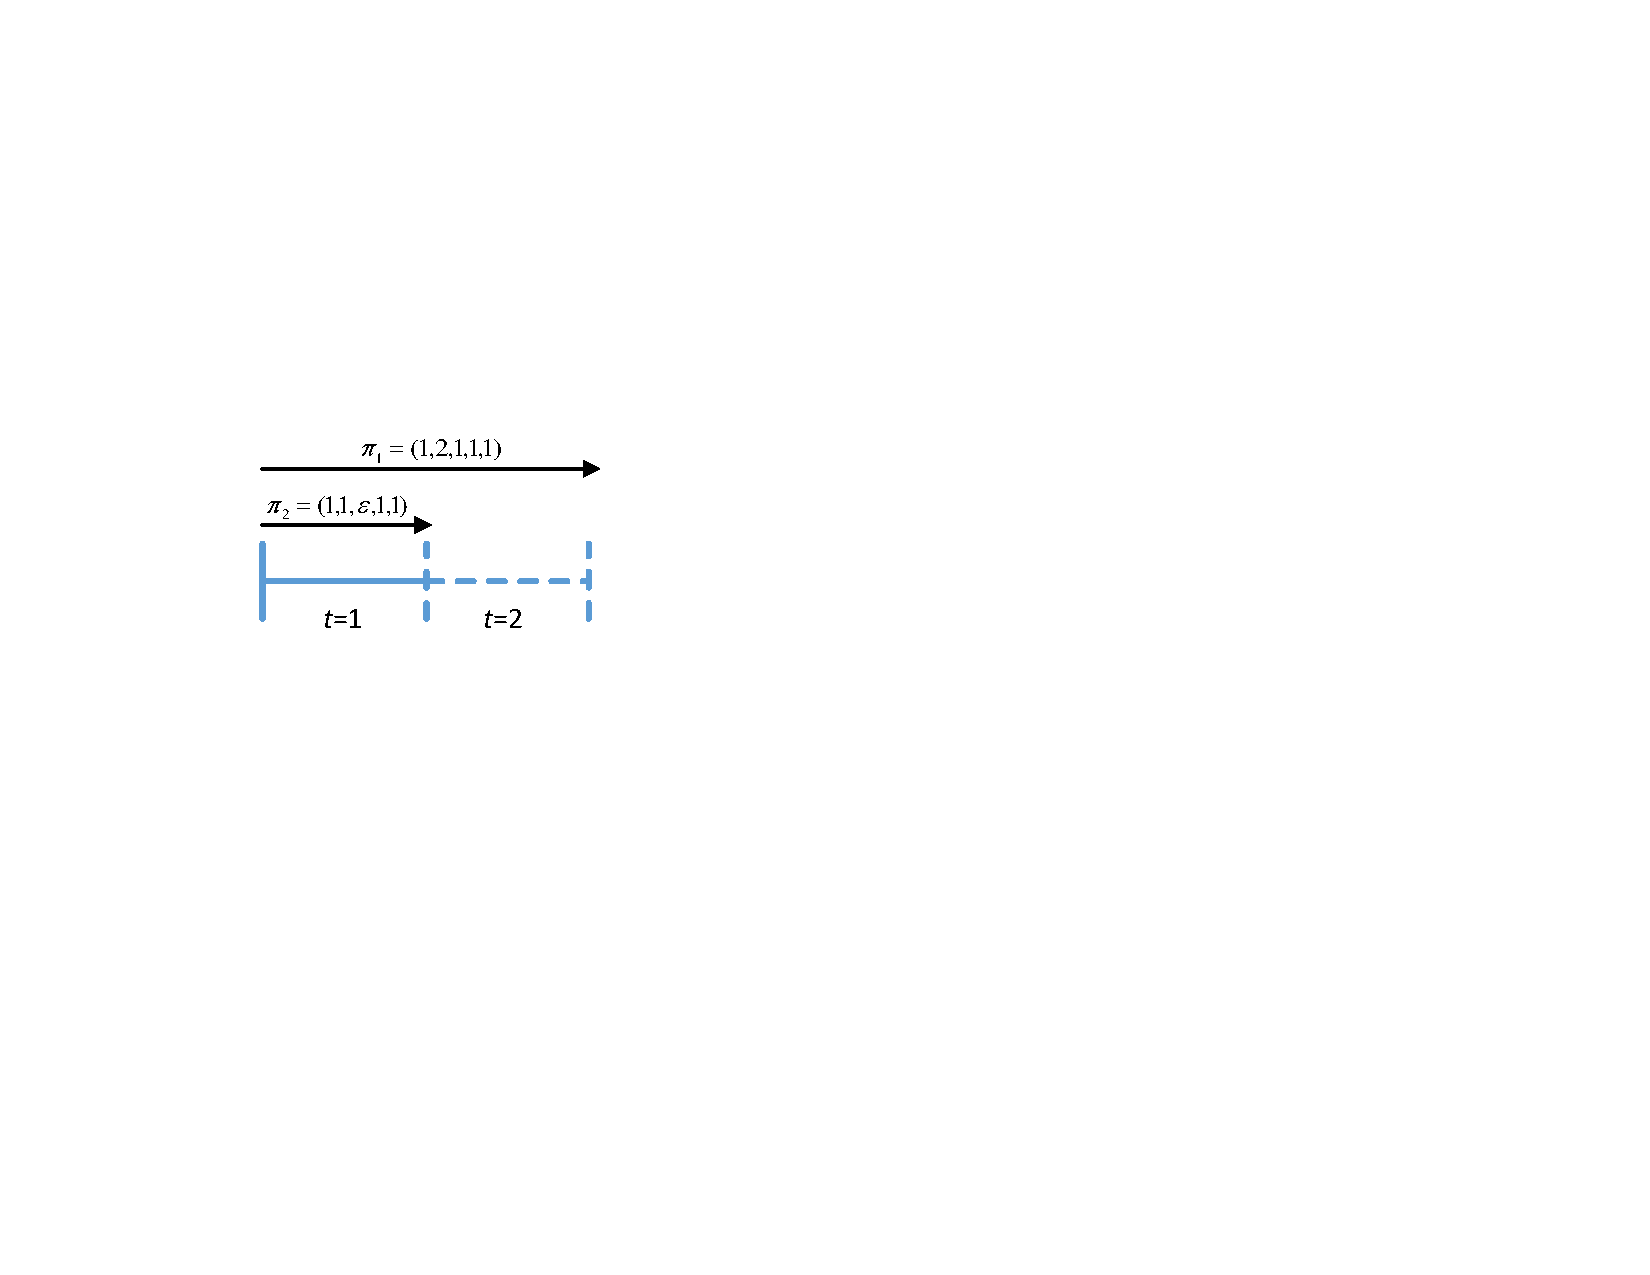
\includegraphics[width=\textwidth]{Ex1a.pdf}
		\caption{EVs $1$ and $2$ arrive at $t=1$.}%
		\label{fig:Ex1a}%
		\end{subfigure}
		\hspace{8mm}
		\begin{subfigure}[b]{.33\textwidth}%
		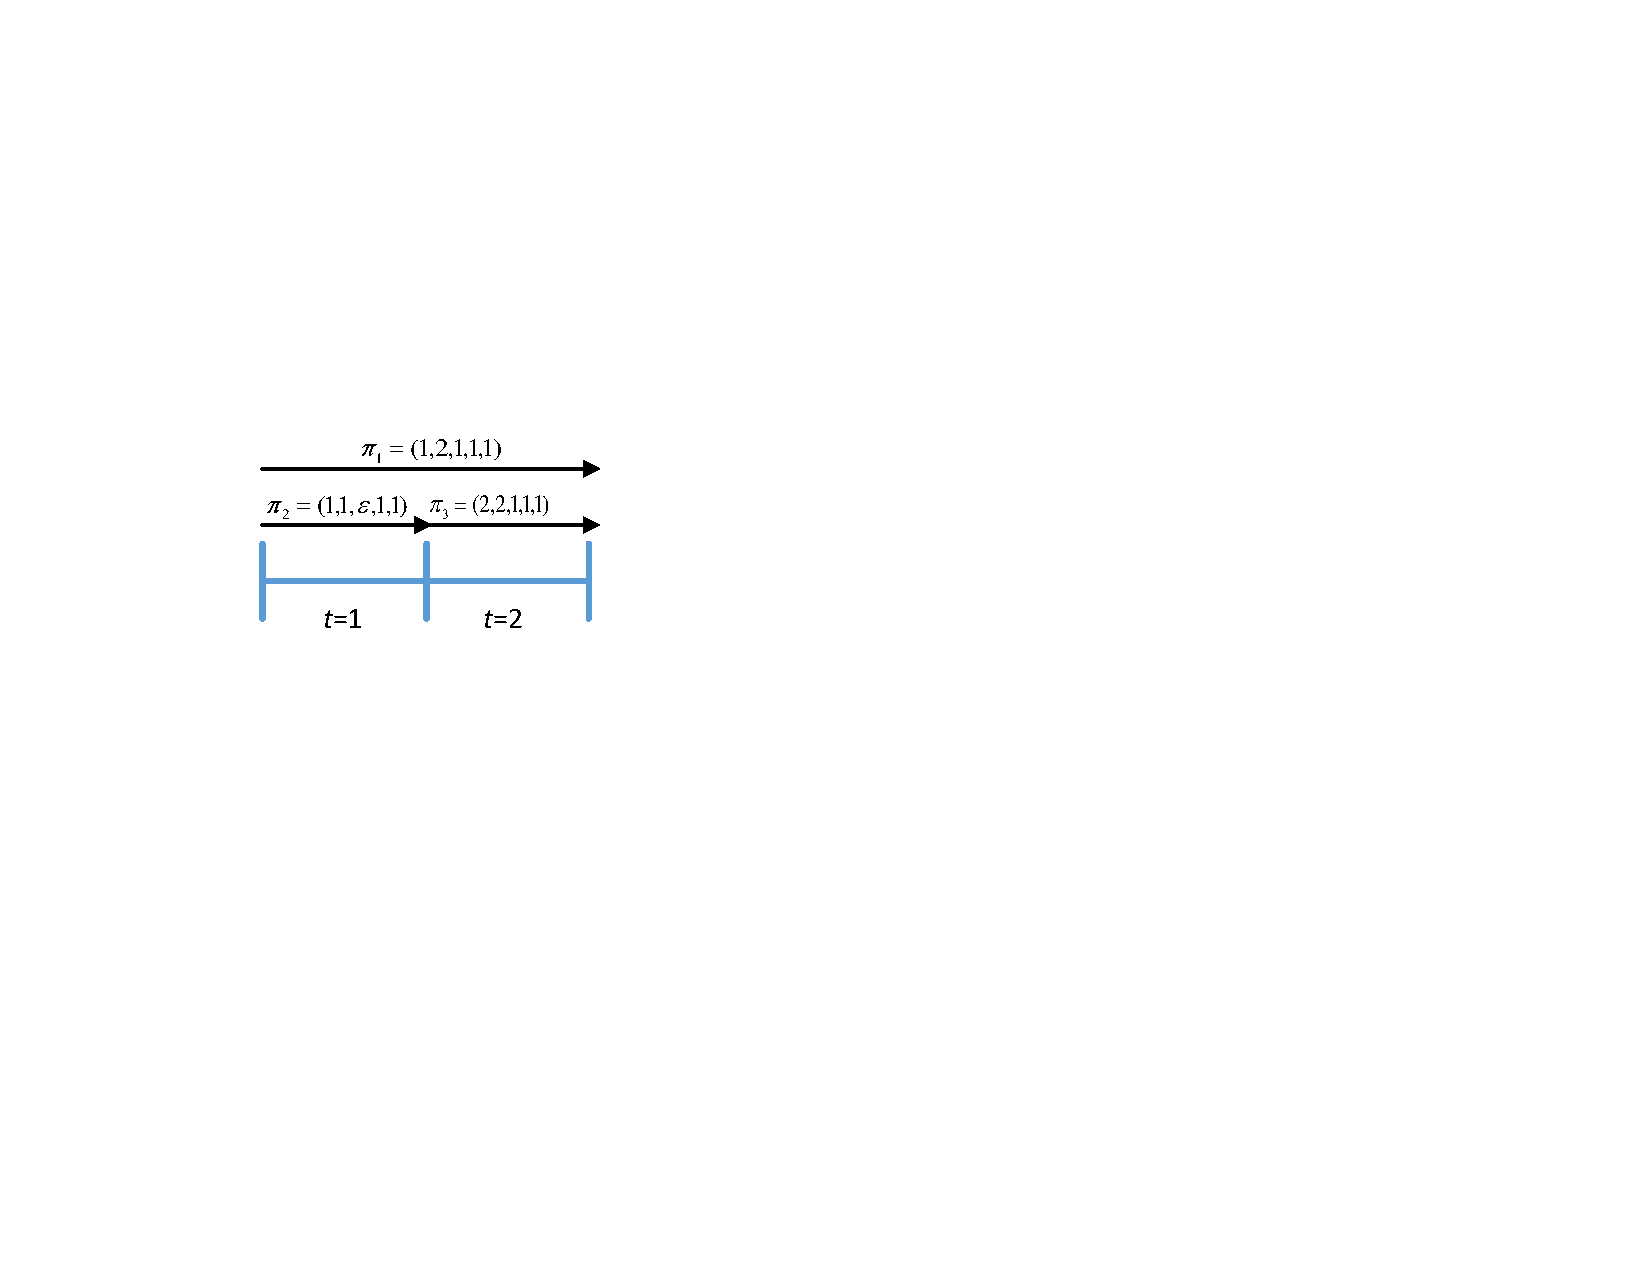
\includegraphics[width=\textwidth]{Ex1b.pdf}
		\caption{EV $3$ arrives at $t=2$.}%
		\label{fig:Ex1b}
		\end{subfigure}		
		\caption{Worst case scenario when the scheduling algorithm is to re-run an optimal algorithm at each time slot considering only available EVs. Dotted line indicates a time slot that is not visited yet and the scheduler has no information about the arriving EVs in that slot. The numbers inside parentheses indicate arrival time, deadline, value, demand and maximum charging rate of the EV, respectively.}
		\label{fig:Ex1}
\end{figure*}

\vspace{5mm}
{
{\color{blue}\noindent\textbf{Comment 1.9:}\\
Page 5 line 21: Please explain the basic algorithm in [18] and how yours is different.
}}

\vspace{5mm}
\noindent\textbf{Response:}

The comment refers to reference [33] in the revised paper which studies the offline problem for integral revenue model in single station scenario. In [33], the authors developed an algorithm which uses the idea of sorting EVs based on their unit value and then select them to charge which is the same general idea we utilized in designing the \ics algorithm. The \ics algorithm extends the proposed algorithm in [33] in three different ways. \textbf{First}, method of [33] works only for single station scenario where there is no global peak constraint. \textbf{Second}, method of [33] works only when arrival times of EVs are the same. \textbf{Third}, we extended theoretical results in [33] and derive performance bounds for the \ics under multiple station scenario. We explained these differences in Section V-A1, Page 7, in the revised manuscript. Last but not the least, we compared the result of our algorithm with the proposed algorithm in [33] as reported in Fig. 3 of the manuscript in Page 9.
\\

\vspace{5mm}
{
{\color{blue}\noindent\textbf{Comment 1.10:}\\
(8a) What is alpha, gamma, beta, pi? How are they related to (1a)-(1d)?
}}

\vspace{5mm}
\noindent\textbf{Response:}

Our solution approach for offline integral revenue model is to develop a primal-dual algorithm which requires formulating the dual problem to analyze the performance using weak duality property. 
Basically, in primal-dual approximation algorithm design, each constraint (resp. variable) in primal (resp. dual) problem is associated with a variable (resp. constraint) in dual (resp. primal) problem. In our case, constraints (1a)-(1d) are respectively associated with dual variables $\alpha, \beta, \gamma$ and $\pi$. For more details, we refer to Chapter 12 of ``Approximation Algorithms'' textbook by Vijay Vazirani, which is cited in our paper as reference [16]. We added a short explanation before formulating the dual problem in Page 6 of the paper. 
\\

\vspace{5mm}
{
{\color{blue}\noindent\textbf{Comment 1.11:}\\
Page 5 line 30: How is the feasibility checked?
}}

\vspace{5mm}
\noindent\textbf{Response:}

The comment refers to feasibility check of allocating an EV in \ics algorithm (Section V-A-1, Page 7, Scheduling of the Selected EV). Since \ics is working under integral revenue model, each EV should receive all or nothing of its demand. Therefore, when \ics is trying to allocate an EV, it should first check that if there is enough remaining resource in availability window of the EV. This check is done in Line 6 of the \ics algorithm in Page 7 of the revised version. \rev{We also cited the corresponding algorithm line  when we used the term ``feasibility check'' in Page 7.} 
\\

\vspace{5mm}
{
{\color{blue}\noindent\textbf{Comment 1.12:}\\
The definition of m and n are very confusing. In the fractional model, the summations are used with n all the time, suggesting that every car will have a charging station. In the integral model (8a), m and n come in together without clear explanation what each term means. 
}}

\vspace{5mm}
\noindent\textbf{Response:}

Parameter $n$ is the total number of EVs (in the entire charging network) and $m$ is the number of charging stations as explained in Table I in Page 3. Each charging station (CS) is equipped with enough number of chargers to charge multiple EVs simultaneously as long as the peak constraint is respected. Moreover, $h(i)$ indicates the charging station of EV $i$ and is given to the problem as an input (i.e., we assume that EVs choose their charging stations). 
We further clarified the explanations in Table I and corresponding explanations in Sections III-A1 and III-A2, in Page 3.

The objective function in (8a) is in the form of $A+B+C$ with $A=\sum_{i=1}^n D_i\alpha _i, B=\sum_{j=1}^m \sum_{t=1}^T p_j\beta (t)$ and $C=\sum_{t=1}^T p^\mathsf{total}\gamma (t)$. 
The term $A$ is constructed according to Constraint (1a) in primal problem which applies the constraint for all $n$ EVs. Therefore, the summation index is $n$. The term $B$ is constructed according to Constraint (1c) which enforces the constraint for all charging stations and all time slots. Therefore, indexes in $B$ are $m$ and $T$ (number of time slots). Similarly, the term $C$ is constructed based on constraint (1b) which applies for all time slots and therefore the summation index in $C$ is $T$.

%Therefore, the studied scheduling problem does not include assignment of EVs to CSs as we assume that there is no communication between users and the scheduler before they arrive to a CS. With these assumptions (which represent a realistic scenario), some CSs might face high amount of power demand while there are few EVs in the other CSs. To handle this situation and achieve a high resource utilization in the charging network, we assumed that local peaks in each CS can be over-provisioned. We note that arriving an EV to a charging stations does not guarantee that it will get charged.  

\vspace{3mm}
{\color{blue}In the case study, the CS number is set and the number of the cars is increased. It's unclear what the authors are doing here? Are all cars guaranteed a CS? If so, what's the point of number of CS? } 

\vspace{3mm}
\noindent\textbf{Response:}

As explained in response to the previous comment, several EVs can get charged in each charging station. Given a fixed number of CSs, we can increase the number of EVs. In the simulation scenario, $n$ EVs randomly select their CSs in the ACN. Therefore, when $n$ increases, the density of EVs at each CS will be increased as well and the algorithms will face resource shortage. The goal is to evaluate the proposed algorithms when the demand-to-supply ratio increases.
%We added a phrase to the simulation setup to clarify this. 

\vspace{3mm}
{\color{blue}If CS defines the bottleneck of maximum vehicle charging at the same time, what are the other cars doing? Waiting? But in Fig. 2 and 3, the revenue with different number of CS (and quite small compared to 100 cars) are almost the same. Nothing is explained clearly.}

\vspace{3mm}
\noindent\textbf{Response:}

We thank the reviewer for pointing this issue. Fig. 2 and Fig. 3 are combined in the revised paper due to space limit. 

We highlight two points here. First, in our system model, if the CS cannot charge all EVs in the station simultaneously according to the peak constraints, some EVs should wait. When EV $i$ is waiting, we have $y_{i,t}=0$. However, the scheduler can switch between different subset of EVs for charging. Particularly, preemption is allowed with no cost i.e., the scheduler can pause charging of an EV and resume it later.

Second, since both local and global peak constraints must be respected by the scheduling algorithms, adding more charging stations (with known local peak constraints) may not lead to a revenue improvement if the global peak constraint is not increased accordingly. %Therefore, to increase the revenue of the ACN, increasing the number of CSs is not enough if the global peak constraint is fixed and acts as the bottleneck. 
This is the main reason that the revenue of the algorithms do not greatly improve by increasing number of CSs in Fig. 2 of the previous submission. In the revised paper, we updated our simulation setting and re-run all the scenarios. It can be observed from Fig. 2 of the revised paper that by increasing the number of CSs, the revenue also increases.

%This is the main reason that revenue in Fig. 2 and Fig. 3 is almost the same. To make the scenario meaningful, we re-run the simulation by choosing a higher value of global peak constraint and based on the new result, the total revenue increased as number of CSs increases. 


\vspace{5mm}
{
{\color{blue}\noindent\textbf{Comment 1.13:}\\
Table III: The max charging rate for EVs are largely wrong. It's well known that a Tesla can charge up to 120kW with DC and CHAdeMO (Nissan Leaf)/J1772 Combo (BMW) can charge at 30kW/60kW.
}}

\vspace{5mm}
\noindent\textbf{Response:}

The charging rates we used in the first submission were not up-to-date according to the latest battery technologies. 
In light of this comment, we updated the rates by assuming that DC chargers are installed in the charging stations and the charging method is CHAdeMO which can give a charging rate up to 50 kW. We re-run all the simulations accordingly and  reported the new results. 
% kWh is a measure of energy while kW is a measure of power. That is to say, the unit should be kWh when we are talking of ``storage'' (e.g., battery capacity) while it should be kW when talking of charging/discharging ``rate''.

\vspace{5mm}
{
{\color{blue}\noindent\textbf{Comment 1.14:}\\
Page 7 line 39-41: The setup of the case study is very unclear. We don’t know how many cars are coming at what time, how long they stay and what energy they typical ask for. The revenue of the two cases are almost the same (up to ~10\% difference), which means that the resources in the case study are mostly enough for the demand. This might not be an interesting case especially for the integral revenue case. The author should investigate more deeply how the performance would be different when the supply is not enough (with more and more vehicles). 
}}

\vspace{5mm}
\noindent\textbf{Response:}

We thank the reviewer for pointing this issue.
We revised the simulation set up and made it clear how we set EVs' profile including their demand, deadline and valuation. For details, please see \emph{Simulation Setup and Overview} in Section VI, Page 8. Also, we set local and global peak constraints in our main simulation scenario in Fig. 2 of the paper (Section VI, Evaluation Based on Total Revenue) such that the algorithms face resource shortage. To show the level of the resource scarcity in the new setting, in Fig. 2 of this letter fraction of the fully charged EVs in different methods extracted from the simulation data of Fig. 2 in the paper. As it can be seen from Fig. \ref{fig:acc} in this letter,
even in optimal solution and for the case of having $8$ CSs, the percentage of the EVs who received their entire demand is less than $65\%$ which implies a high level of resource shortage. Due to space constraint, we do not report the results in Fig. \ref{fig:acc} in the manuscript.

We re-run all the simulations with the new setting and reported the results in the paper. Based on the new results in Fig. 2 of the paper in Page 9, we observe that when the number of CSs increases (specially from 2 to 4) by keeping the global peak constraint fixed, the revenue of the algorithms increases as well for all methods.

\begin{figure*}[t]	
				\centering
				\begin{subfigure}[b]{0.3\textwidth}
					\begin{center}
						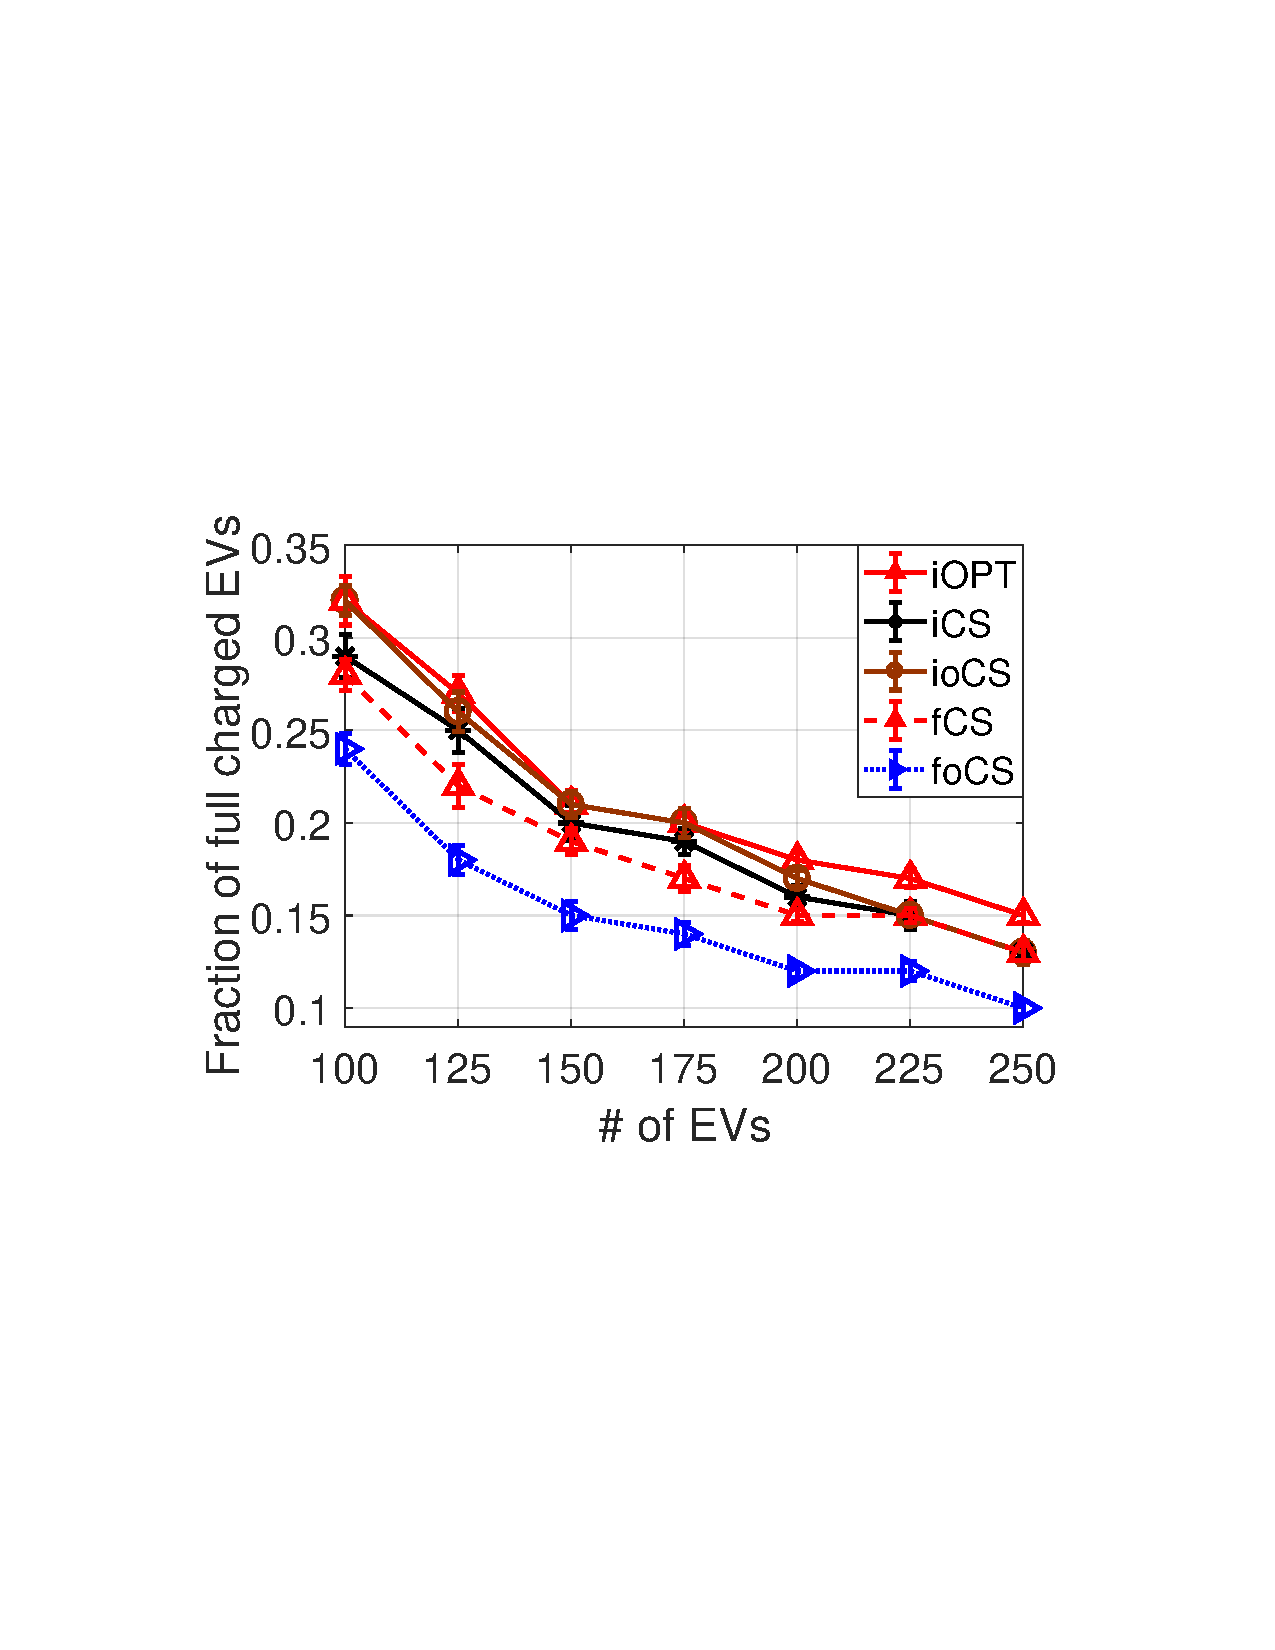
\includegraphics[width=\textwidth]{acc-M2.pdf}
						\caption{$m=2$}
						\label{fig:acc-M2}
					\end{center}
				\end{subfigure}
				\begin{subfigure}[b]{0.3\textwidth}
					\begin{center}
						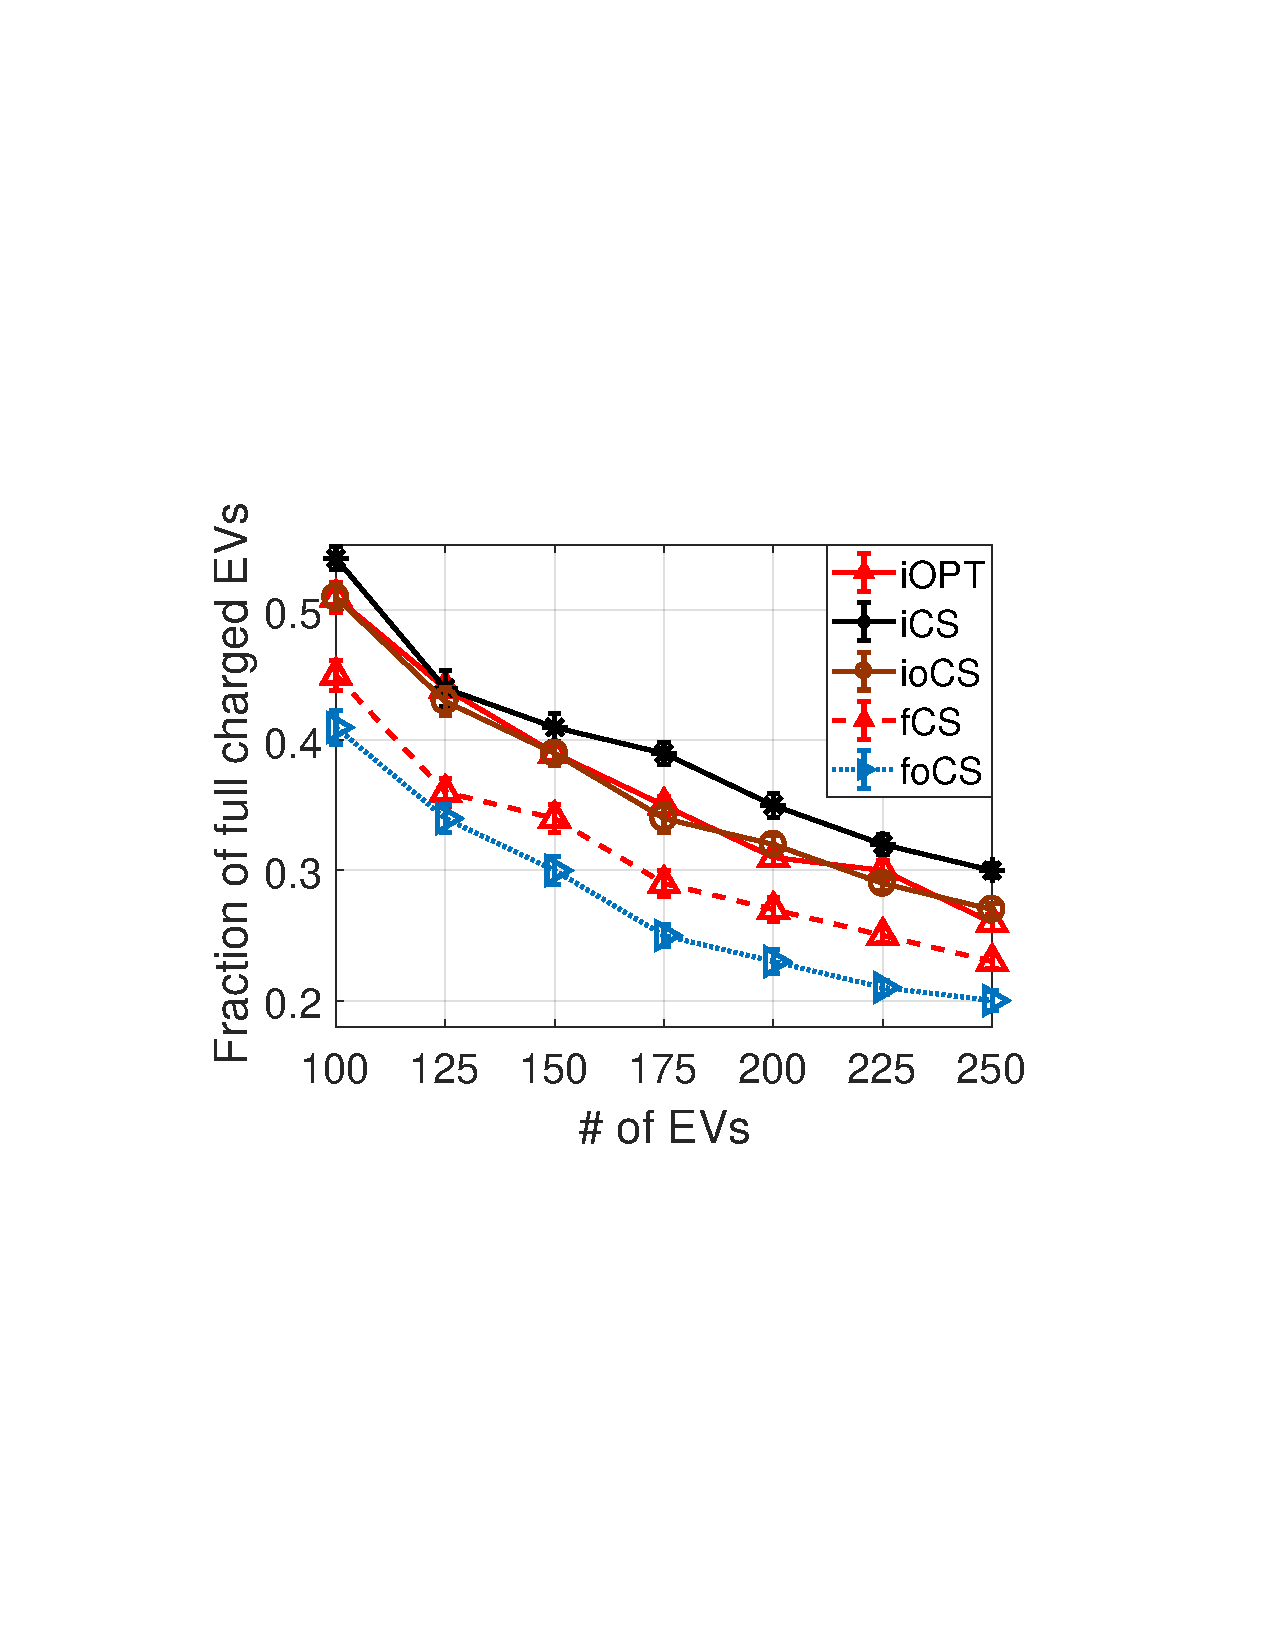
\includegraphics[width=\textwidth]{acc-M4.pdf}
						\caption{$m=4$}
						\label{fig:acc-M4}
					\end{center}
				\end{subfigure}% 	
				\begin{subfigure}[b]{0.3\textwidth}
					\begin{center}
						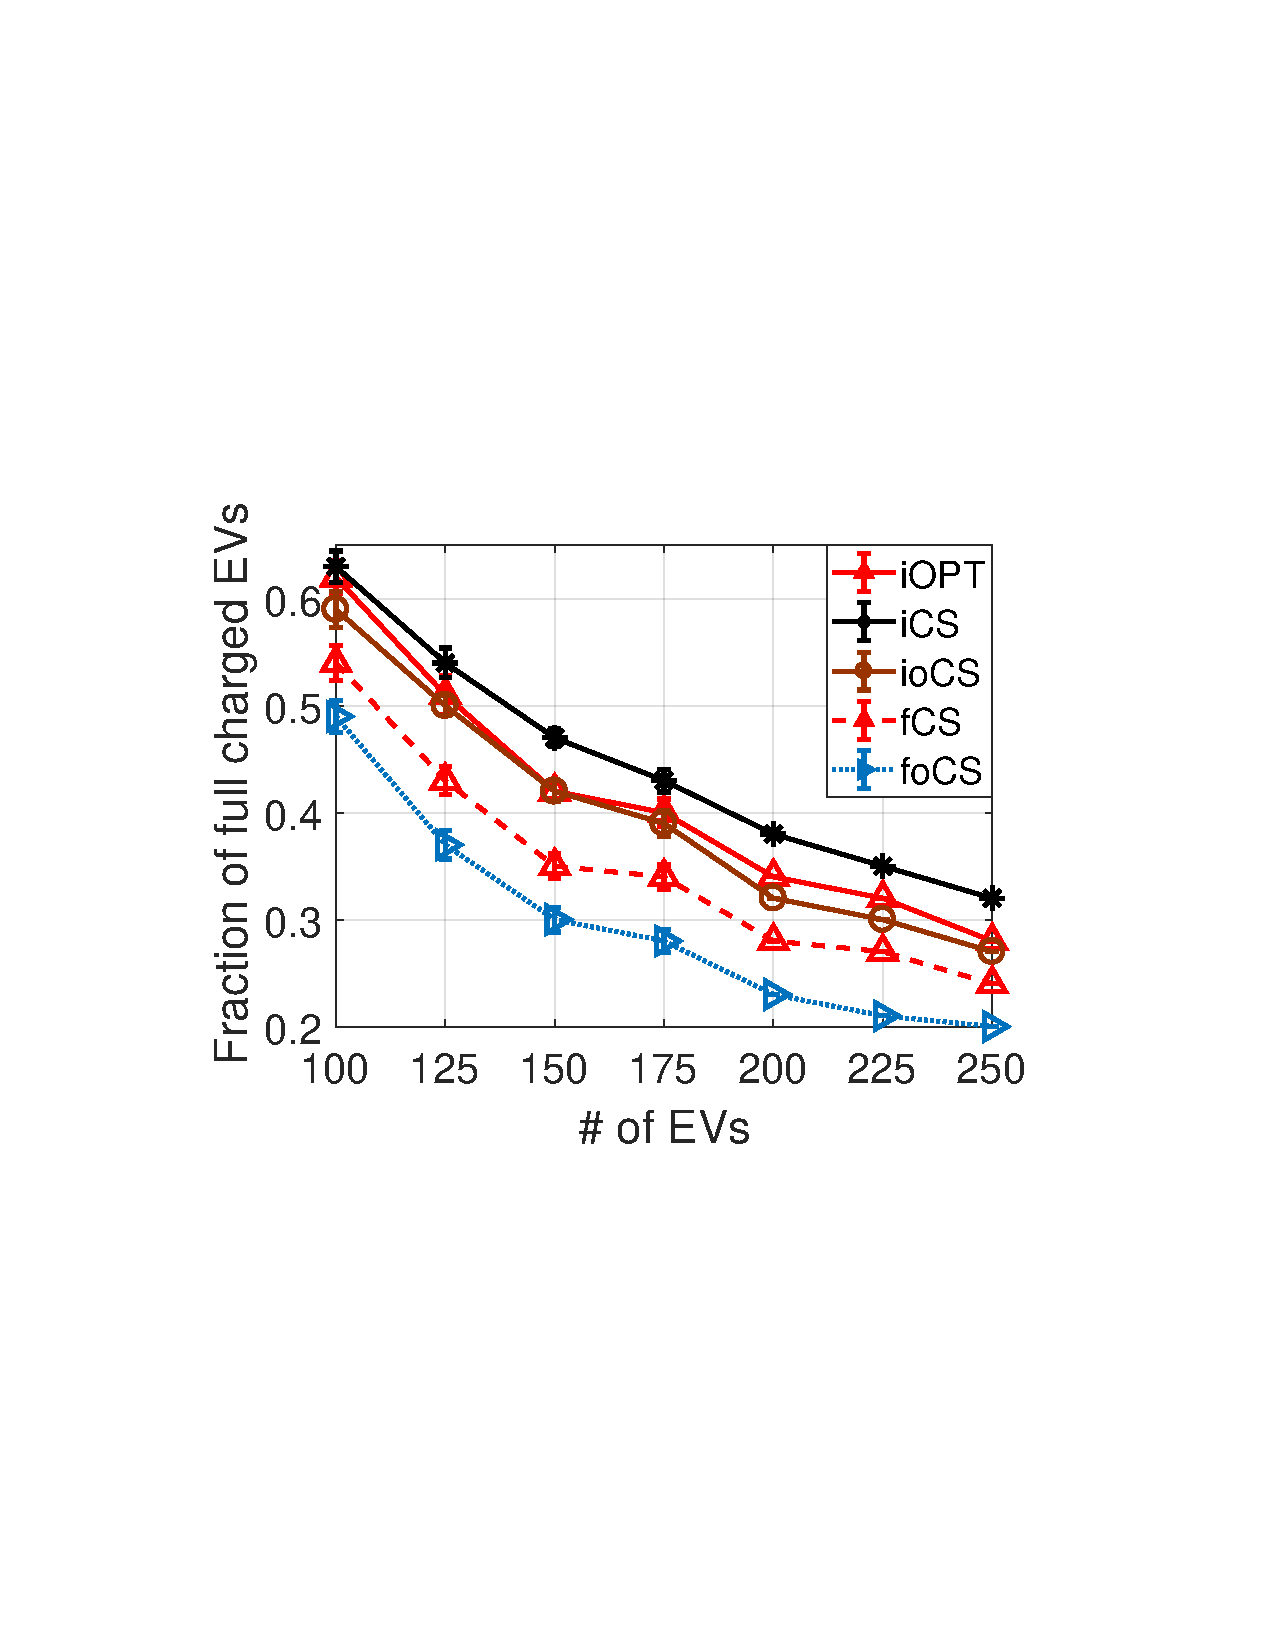
\includegraphics[width=\textwidth]{acc-M8.pdf}
						\caption{$m=8$}
						\label{fig:acc-M8}
					\end{center}
				\end{subfigure}% 
				\caption{Fraction of full charged EVs in different methods.} 
				\label{fig:acc}
				\vspace{-3mm}
			\end{figure*}

 

\vspace{5mm}
{
{\color{blue}\noindent\textbf{Comment 1.15:}\\
Fig 2, 3: With more and more vehicles, both scenarios should show a converged non-linear revenue curve, with the integral revenue converging more pre-maturely. But the shown result is simply linear, again showing that the capacity is not saturated and the case study is ill set-up.
}}

\vspace{5mm}
\noindent\textbf{Response:}

We agree with the reviewer that after some point and when number of EVs is large compared to the available resources, increasing the number of EVs should not change the total revenue obtained by the algorithms mainly because the newly added EVs cannot make a difference in solution of the algorithms. In our new simulations, this can be seen in Fig. 2a in the revised version where the revenue of the different algorithms only slightly change when number of EVs is increasing from 200 to 250. This is not the case in Fig. 2b and Fig. 2c of the paper. However, it is not because the capacity is not saturated as the reported results in Fig. \ref{fig:acc} of this letter shows that there is a great amount of resource shortage. We believe that the reason lies behind the heterogeneity of EVs' unit value. When increasing number of EVs, until some point, the algorithms are able to improve their selected EVs for charge by relying on EVs with higher unit values \emph{while probably leaving a large portion of EVs un-allocated.} Therefore, the fact that the revenue is linearly increasing in Fig. 2b and Fig. 2c of the paper with the number of EVs does not imply that the capacity is not saturated. 
We believe that if we increase number of EVs in a highly dense scenarios, the revenue of the algorithms will only change slightly with different number of EVs. \rev{To investigate this, we re-run the scenario of Fig. 2 of the revised manuscript while the number of EVs is increased from 400 to 500 instead of 100 to 250 and plotted the results in Fig. \ref{fig:V-NN} in this letter. Based on the results, there is no significant improvement in highly dense scenarios which confirms our argument.} However, this result confirms a simple fact and does not address our simulation goal in Fig. 2 of the paper which is observing how the algorithms scale with the number of EVs.


\begin{figure*}[t]	
				\centering
				\begin{subfigure}[b]{0.3\textwidth}
					\begin{center}
						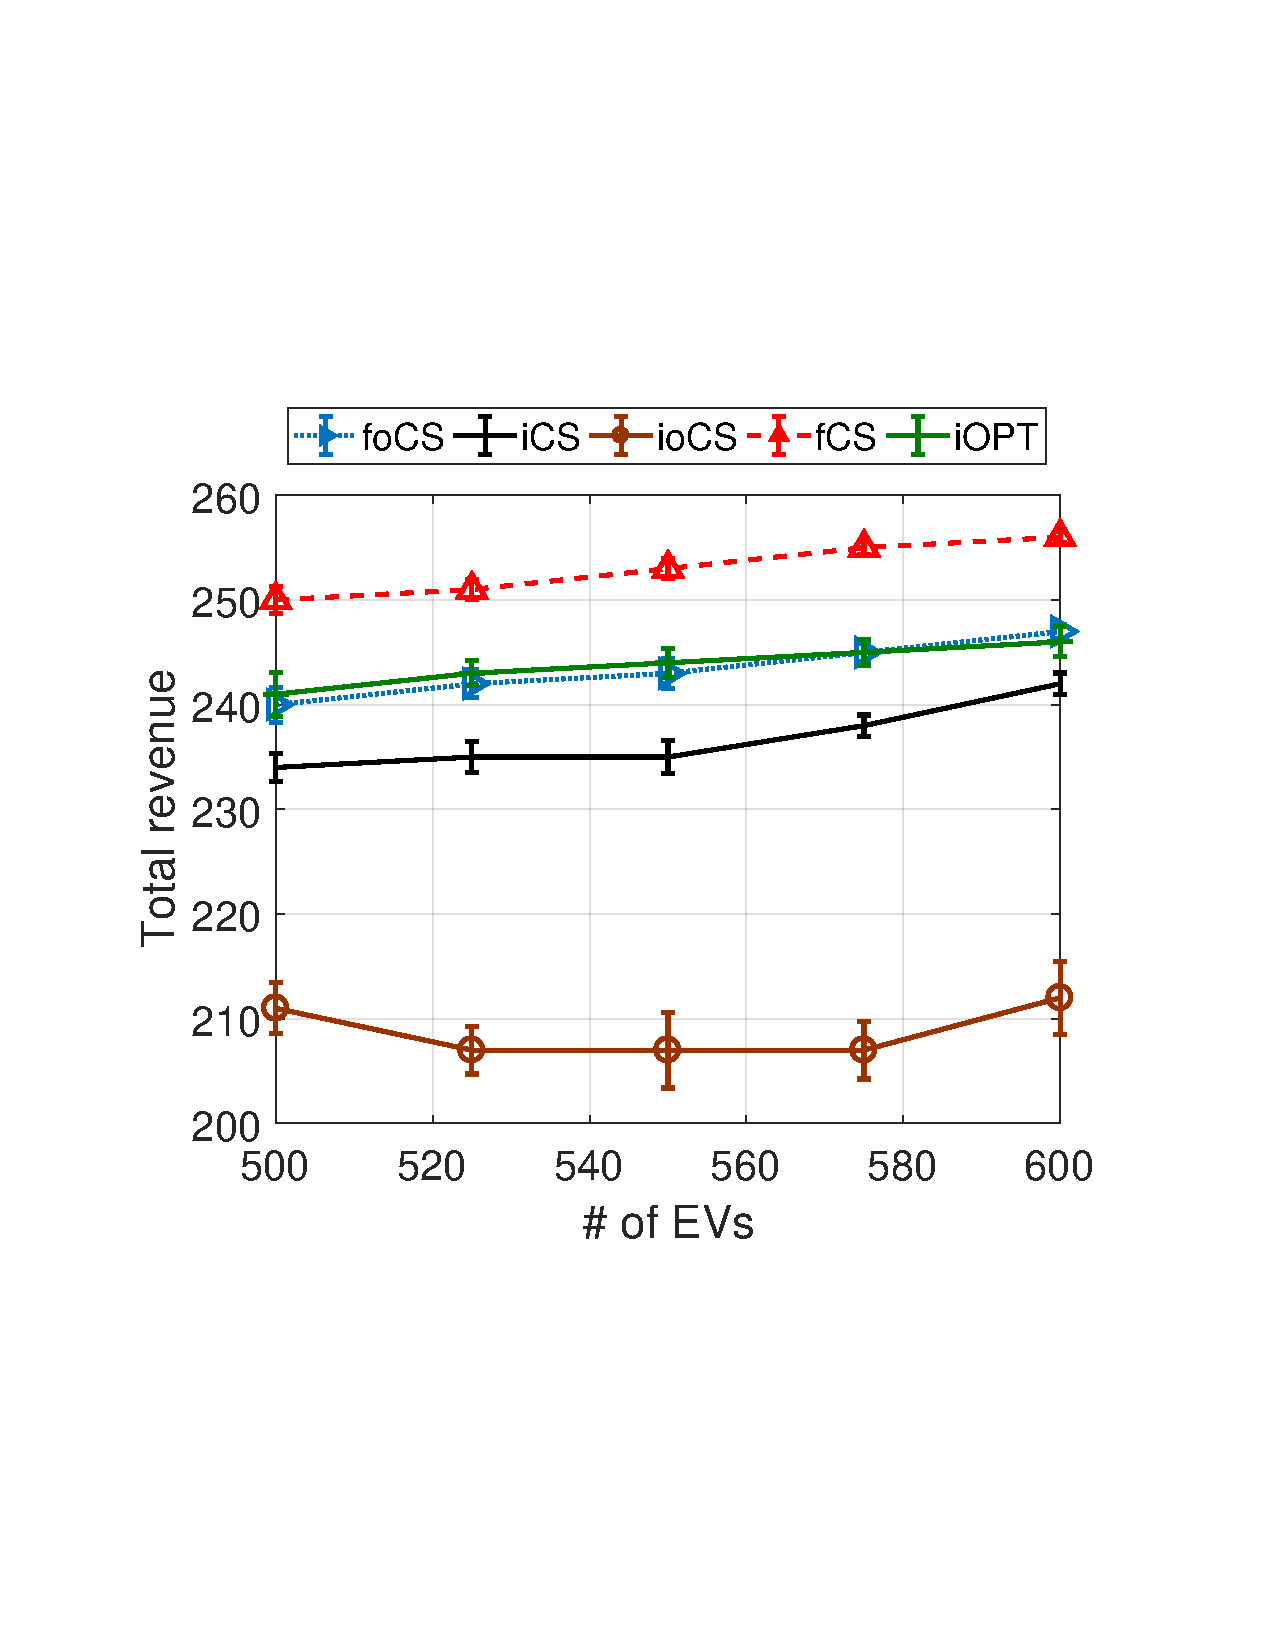
\includegraphics[width=\textwidth]{V-NN2.pdf}
						\caption{$m=2$}
						\label{fig:V-NN2}
					\end{center}
				\end{subfigure}
				\begin{subfigure}[b]{0.3\textwidth}
					\begin{center}
						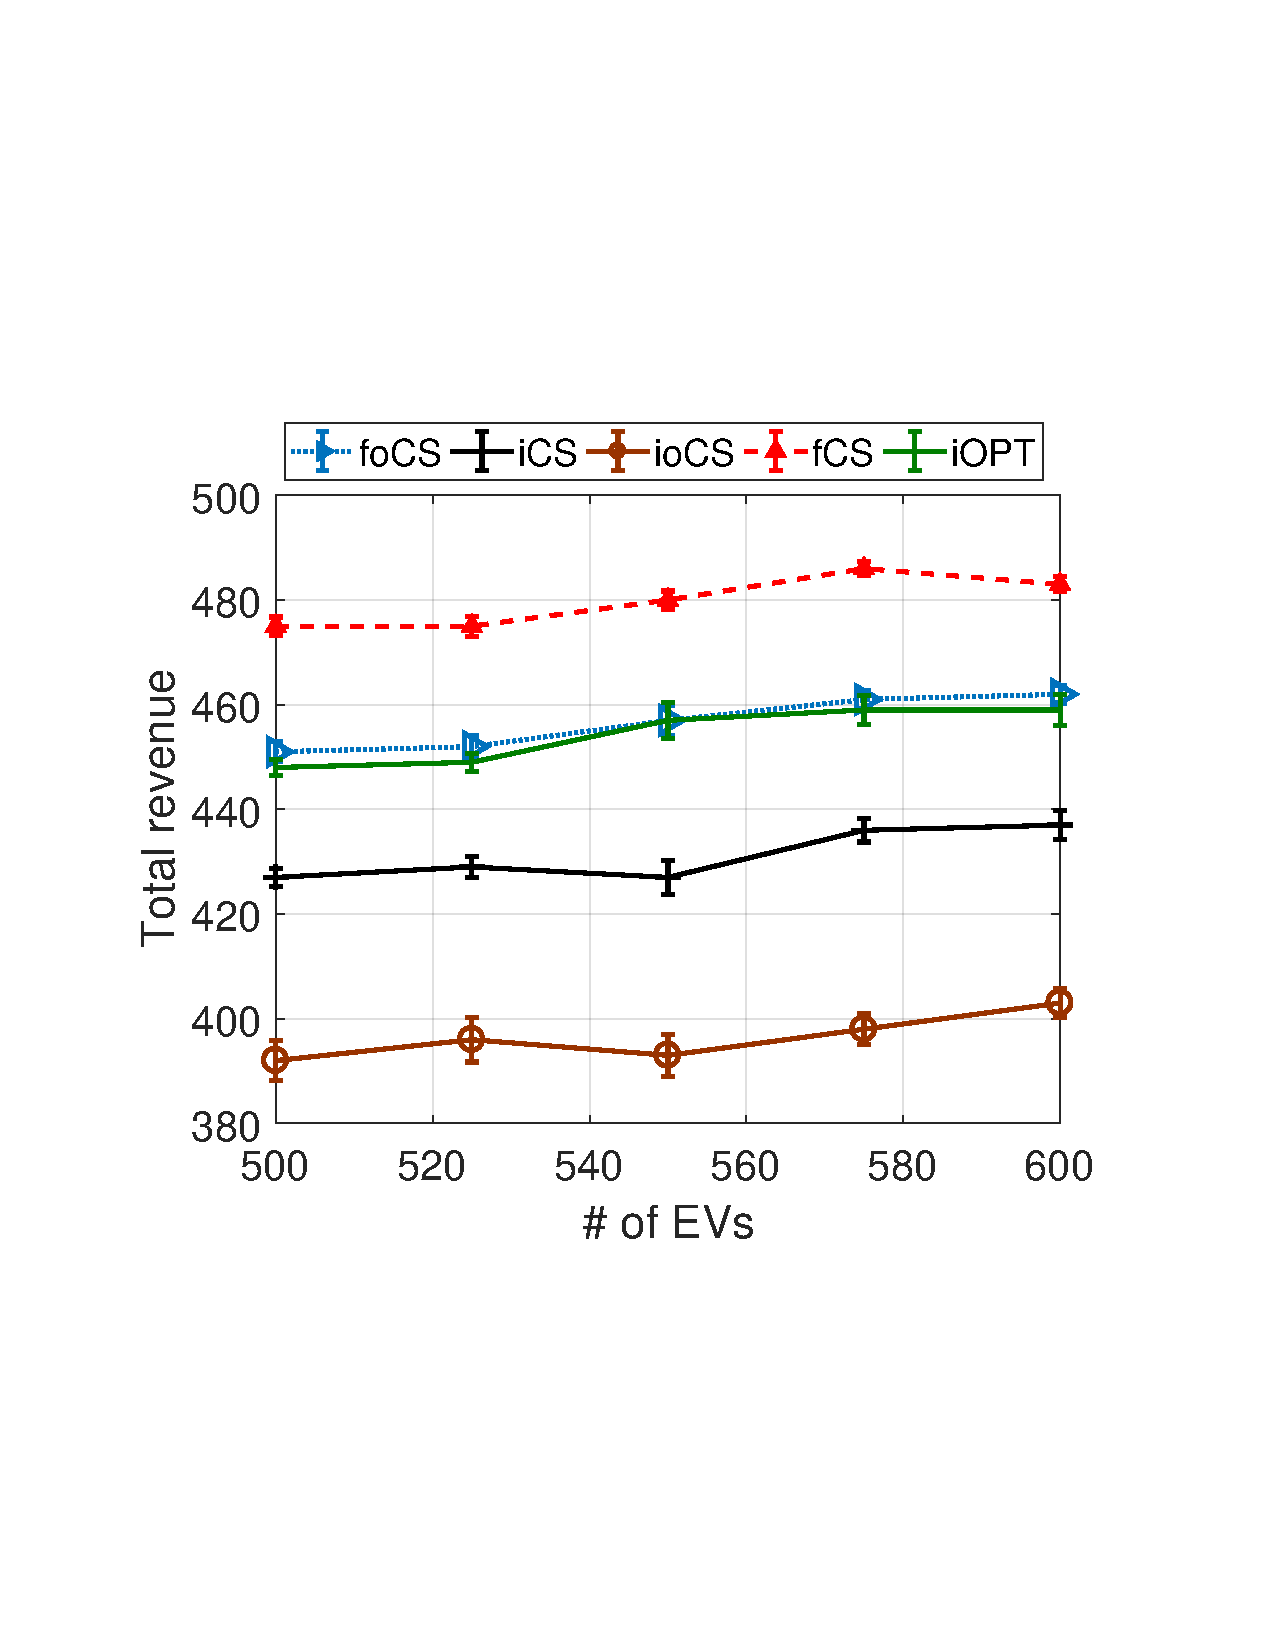
\includegraphics[width=\textwidth]{V-NN4.pdf}
						\caption{$m=4$}
						\label{fig:V-NN4}
					\end{center}
				\end{subfigure}% 
				\caption{Investigating the impact of increasing number of EVs in highly dense scenarios.} 
				\label{fig:V-NN}	
			\end{figure*}

\vspace{5mm}
{
{\color{blue}\noindent\textbf{Comment 1.16:}\\
How the valuation is generated for each user in the case study is not explained.
}}

\vspace{5mm}
\noindent\textbf{Response:}

We thank the reviewer for pointing this issue. The unit value of each EV in the simulation is randomly and uniformly selected from interval $[\frac{1}{2}z,\frac{3}{2}z]$ where $z$ is average price for 1 kWh of power in the US. We added this explanation to simulation setup in Section VI.

\vspace{5mm}
{
{\color{blue}\noindent\textbf{Comment 1.17:}\\
The author should consider customer’s satisfaction in the optimization. User’s demand is only used to determine whether it’s feasible, rather than giving their priorities. It would seem too brutal to reject/rank users solely by how much they try to pay.
}}

\vspace{5mm}
\noindent\textbf{Response:}

The variable $v_i$ provides us with enough flexibility to handle such scenarios. 
Let's assume that the overall satisfaction of a user is determined using a function $f(.)$ of multiple parameters (e.g., their payment, priority, etc) where the output of $f(.)$ for profile of user $i$ is $v_i$. Then, our formulated optimization problem turns into maximizing the overall satisfaction of the users while there is no modification required in the proposed algorithms. 


%%%%%%%%%%%%%%%%%%%%%%%%%%%%%%%%%%%%%%%%%%%%%%%%%%%%%%%%%%%%%%%%%%%%%%%%%%%%%%
%%%%%%%%%%%%%%%%%%%%%%%%%%%%%%%%%%%%%%%%%%%%%%%%%%%%%%%%%%%%%%%%%%%%%%%%%%%%%%
%%%%%%%%%%%%%%%%%%%%%%%%%%%%%%%%%%%%%%%%%%%%%%%%%%%%%%%%%%%%%%%%%%%%%%%%%%%%%%
%%%%%%%%%%%%%%%%%%%%%%%%%%%%%%%%%%%%%%%%%%%%%%%%%%%%%%%%%%%%%%%%%%%%%%%%%%%%%%
%%%%%%%%%%%%%%%%%%%%%%%%%%%%%%%%%%%%%%%%%%%%%%%%%%%%%%%%%%%%%%%%%%%%%%%%%%%%%%
%%%%%%%%%%%%%%%%%%%%%%%%%%%%%%%%%%%%%%%%%%%%%%%%%%%%%%%%%%%%%%%%%%%%%%%%%%%%%%
%%%%%%%%%%%%%%%%%%%%%%%%%%%%%%%%%%%%%%%%%%%%%%%%%%%%%%%%%%%%%%%%%%%%%%%%%%%%%%
%%%%%%%%%%%%%%%%%%%%%%%%%%%%%%%%%%%%%%%%%%%%%%%%%%%%%%%%%%%%%%%%%%%%%%%%%%%%%%
%%%%%%%%%%%%%%%%%%%%%%%%%%%%%%%%%%%%%%%%%%%%%%%%%%%%%%%%%%%%%%%%%%%%%%%%%%%%%%
%%%%%%%%%%%%%%%%%%%%%%%%%%%%%%%%%%%%%%%%%%%%%%%%%%%%%%%%%%%%%%%%%%%%%%%%%%%%%%
%%%%%%%%%%%%%%%%%%%%%%%%%%%%%%%%%%%%%%%%%%%%%%%%%%%%%%%%%%%%%%%%%%%%%%%%%%%%%%
\newpage
\section{Reviewer $\# 2$}
{\color{blue}}
%
%\vspace{4mm}
%{\color{blue}\noindent\\
%We sincerely appreciate you for taking the time to review
%our paper. Following the concerns and suggestions, the paper
%has carefully been revised to address the reviewer's comments
%properly.
%}

%We sincerely appreciate you for taking the time to review our paper. Following the
%concerns and suggestions, the paper has carefully been revised to address the reviewer's
%comments properly. 

{\color{blue}This paper considers a EV charging problem with both local and global maximum charging rates. Considering both fractional and integer charging control problems, this paper proposed a offline and an online algorithm for each problem.}

\subsection{Comments}

\vspace{5mm}
{
{\color{blue}\noindent\textbf{Comment 2.1:}\\
The paper intends to include four algorithms in one paper under strict 8-page limit. As a result, even important literature reviews on online algorithm design are moved to the appendix, which is not a common practice and in fact a bad way to present the paper to the audience. The offline algorithm for the fractional case is not described at all in the paper, but referring to an online report. As a result, the paper is not self-contained in its current form.
}}

\vspace{5mm}
\noindent\textbf{Response:} 

In the revised manuscript, we complied a 10-page manuscript by reorganizing the paper and adding several important contents to the main body of the paper to make it self-contained. In particular, we added the \rev{Related Works section} and optimal offline algorithm from our technical report to the revised manuscript, with detailed explanations, hence in the revised version there is no more algorithms cited from other references. The details of this algorithm is in Section IV-A, Pages 4-5 of the revised manuscript. 
\\


\vspace{5mm}
{
{\color{blue}\noindent\textbf{Comment 2.2:}\\
Compared to the existing solution without the global constraint, that is the new challenge in the design? Does this greatly impact the algorithm design.
}}

\vspace{5mm}
\noindent\textbf{Response:}

Without the global peak constraint, the problem degenerates to multiple single-station sub-problems, each with a local peak constraint. In this scenario, the global optimal solution can be obtained by solving sub-problems separately. 

In the presence of a global peak constraint where the aggregate capacity constraint of charging stations is greater than the global peak constraint, the optimal solutions of the sub-problems may not be feasible for the global problem. This is because the aggregate demand obtained by optimal local solutions may go beyond the maximum tolerable capacity of the adaptive charging network. Consequently, the problem must be solved globally, by taking into account both local and global peak constraints. 
It is worth to note that this two-level capacity constraint architecture comes from the practical systems. Our motivation in this paper is from Caltech Adaptive Charging Network, where the ACN operator might limit the total power drawn from EVs (which is essentially the global peak constraint) to control costs, reserve the capacity for other loads, and/or participate in demand-response events. 

In terms of algorithm design, the general ideas of sorting and selecting the most valuable sources are still the same as the case without the global peak constraints, however, there are several details in both algorithm design and competitive and approximation analysis where we do required specific design tailored for the case with global peak constraints. In the following, we mention some of the technical challenges by adding global peak constraints:
\begin{itemize}
	\item Additional steps in constructing dual  problem (as appeared in the the third term in the objective function of dual problem in Equation (9a) in Page 6 of the revised manuscript). This leads to additional challenges in weak-duality analysis in primal-dual framework. 
	\item More sophisticated scheduling rules in algorithms design to ensure respecting the global peak constraints (e.g., Line 4 of Algorithm 2, Line 4 of Algorithm 4, etc.). 
\end{itemize}
Last but not the least, we note that our competitive analysis in Section IV-B is entirely novel and to the best of our knowledge is not used in any previous work. 


\vspace{5mm}
{
{\color{blue}\noindent\textbf{Comment 2.3:}\\
We can clearly see in the formulation (1) that the EVs have different charging price $v_i/D_i$. From the system operator's perspective, why serving different users at different prices, is this reasonable and practical in commercial system? or it is just an extension from the Knapsack problem.
}}

\vspace{5mm}
\noindent\textbf{Response:}

This is a constructive comment that also raised by the Reviewer 1 in Comment 1.2. For detailed explanation we refer to our response to Comment 1.2. However, in the following we provide a short response as well. 

In this study, we consider the scenario in which the aggregate EV charging demands are beyond the local and global peak constraints of the adaptive charging network.  In this resource-limited scenario, it is rationale to solve a social welfare maximization problem with the goal of maximizing the aggregate \textit{utility} (in simplified case, \textit{valuation}, as we considered in our paper) of the users, i.e., EVs, in the system. 

In the current scenarios, the aggregate demand is usually lower than the local and global peak constraints,  hence, the charging model pointed by the reviewer makes sense. This flat charging model, however, is not sustainable in the scenarios in which the peak constraints hinders fulfilling the entire demand of the users. As advocated in our study (and several other studies in EV charging scheduling or in broader way in general utility maximization resource allocation problems such as [8], [11], [33] in the revised manuscript), a natural way is to let EVs to announce their willingness to pay and try to propose scheduling mechanisms that maximizes the aggregate valuation subject to the capacity constraints.

\vspace{5mm}
{
{\color{blue}\noindent\textbf{Comment 2.4:}\\
The generalized Knapsack problem must have off-the-shelf efficient approximate methods, the authors should consider comparing the proposed method with them. For the fractional one, what is the advantages of the proposed off-line method compared to general method to solve LP, e.g., interior point method.
}}

\vspace{5mm}
\noindent\textbf{Response:}

First we emphasize that the formulated problem in this study is a time-expanded online version of original knapsack problem, which is more complicated than the basic knapsack problem. Consequently, applying the off-the-shelf approximation methods for knapsack problem may not be possible or may produce unsatisfactory results. Second, in simulations, we compared the results of our proposed online and offline algorithms against optimal solutions where the optimal solution is obtained using Gurobi (reference [38] in the revised paper) as a generic off-the-shelf solver to solve mixed integer linear problems. 

The advantages of the proposed offline algorithm against general methods to solve LPs are (i) it comes with lower computational complexity, and more importantly (ii) it provides insights in designing online algorithm for fractional case, and offline and online algorithms for integral case; and finally, (iii) it leverages a valley-filling policy to further reduce the peak by distributing the demand over time smoothly. 

\vspace{5mm}
{
{\color{blue}\noindent\textbf{Comment 2.5:}\\
What is the point of Fig. 4 if considering only a single charging station where the global peak constraint is absent (the main contribution of this paper)?
}}

\vspace{5mm}
\noindent\textbf{Response:}

Fig. 4 is now Fig. 3 in the revised version as we combined figures to save space.
The goal here is to compare our method to existing works (in particular, GreedyRTL algorithm in reference [33] in the revised paper), and show that even in the absence of the global peak, our algorithms work better than the existing works. Since the GreedyRTL works only in single station scenario (so local and global peaks are the same), we set the number of charging stations to one and assumed that there is no global peak constraint. The result is that not only our designed \ics algorithm slightly improves the GreedyRTL in terms of the revenue, but also greatly reduces the actual peak of the charging station through its valley-filling technique.  

\begin{figure*}[t]
	\center
	\begin{subfigure}[b]{.33\textwidth}%
		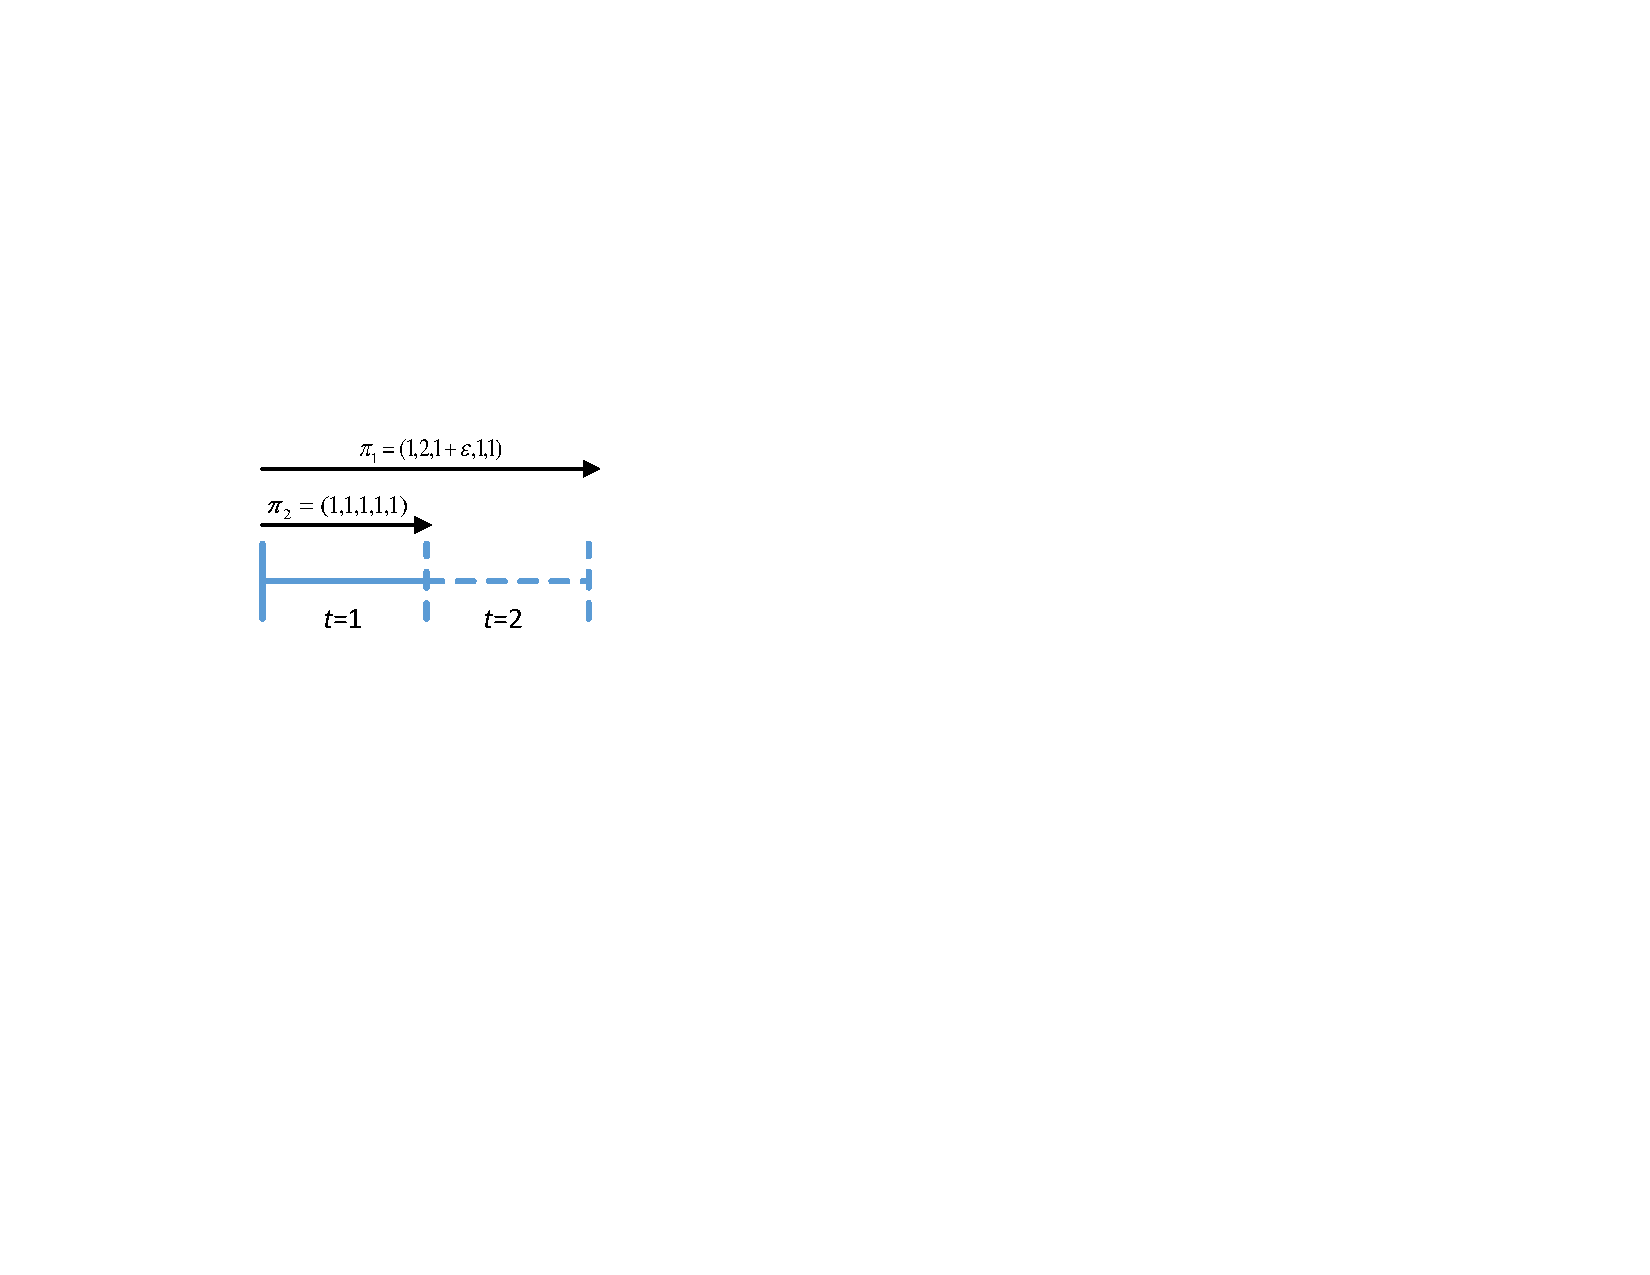
\includegraphics[width=\textwidth]{Ex2a.pdf}
		\caption{Jobs $1$ and $2$ arrive at $t=1$.}%
		\label{fig:Ex2a}%
	\end{subfigure}
	\hspace{8mm}
	\begin{subfigure}[b]{.33\textwidth}%
		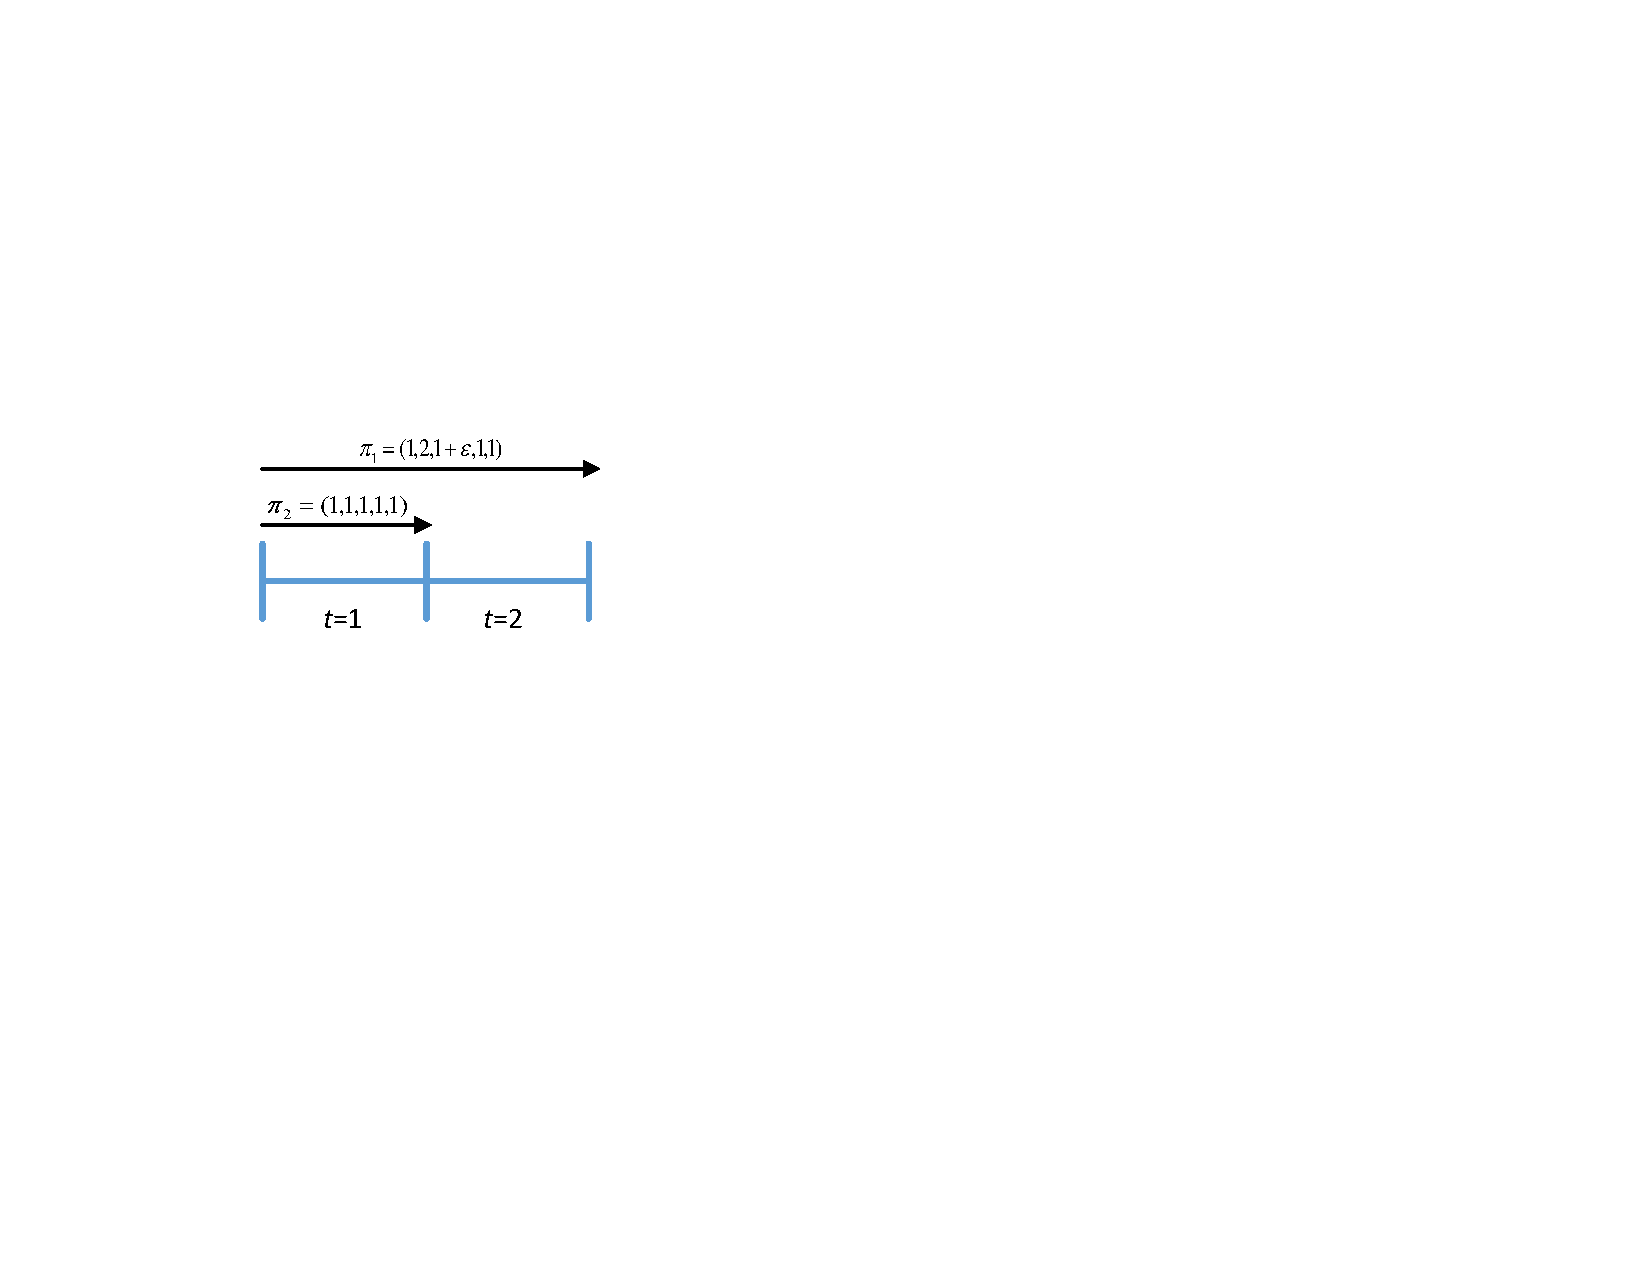
\includegraphics[width=\textwidth]{Ex2b.pdf}
		\caption{No EV arrives at $t=2$.}%
		\label{fig:Ex2b}
	\end{subfigure}		
	\caption{Worst case scenario for the \focs algorithm. Dotted line indicates a time slot that is not visited yet and the scheduler has no information about the arriving EVs in that slot. The numbers inside parentheses indicate arrival time, deadline, value, demand and maximum charging rate of the EV, respectively.}
	\label{fig:Ex2}
\end{figure*}


\vspace{5mm}
{
{\color{blue}\noindent\textbf{Comment 2.6:}\\
In Fig. 2, the proposed foCS performs worse than benchmark foLP, please explain. Besides, the benchmark methods should be briefly explained.
}}

\vspace{5mm}
\noindent\textbf{Response:}

This comment refers to simulation results in the previous version of the paper where the number of EVs is changed from 50 to 100 and revenue results for the algorithms are gathered.
According to the results, \focs performs worse in highly dense scenarios while performs well in low dense scenarios. In the revised manuscript, the simulation settings are fully changed according to Comment 1.14 of Reviewer \#1 to only consider highly dense scenarios which is where the performance of the \focs is below the \folp. We believe that one major reason for this performance issue is that the \focs is \emph{deadline-oblivious} i.e., it does not use the deadline information of the users in decision making. Therefore, in the revised manuscript we made a small but effective modification into the algorithm to make it \emph{deadline-aware} as follows: when algorithm sorts the EVs based on their unit values, if two EVs have the same unit value, then the one with earliest deadline comes first in the sorted list (See Algorithm 2 Lin 2 and the highlighted text in Section IV-B in Page 5). The new simulation results (Fig. 2 in the revised version) show the effectiveness of this method such that the performance of the \focs is now similar or slightly better than the \folp in all cases. 

We also explained the fOLP algorithm in simulation setting in Section VI, Page 9.


\vspace{5mm}
{
{\color{blue}\noindent\textbf{Comment 2.7:}\\
For the competitive analysis, can the authors explain at what condition the worst case (is likely to) happen? Now the 2-competitive result is not surprising and provides little insight.
}}

\vspace{5mm}
\noindent\textbf{Response:}

Fig. \ref{fig:Ex2} in this letter shows the worst case scenario for the \focs algorithm where there is only one charging station with $p_1=p^\text{total}=1$. If we run \focs over the scenario of Fig. \ref{fig:Ex2}, the algorithm will select EV 1 at time slot 1 because its unit value is higher. Then, if no EV arrives at time slot $2$, the total revenue of the algorithm will be $1+\epsilon$ while the optimal solution is to allocate EV 2 at $t=1$ and EV 1 at $t=2$ which makes the total revenue 2. Since we can set the $\epsilon$ to an arbitrarily small value, the competitive ratio is $2$.

We emphasize that this is a theoretical analysis that characterizes the performance of our algorithm in worst-case scenarios. Our simulations results show that in reality the result of our algorithm is much better than worst-case analytical results. 


%%%%%%%%%%%%%%%%%%%%%%%%%%%%%%%%%%%%%%%%%%%%%%%%%%%%%%%%%%%%%%%%%%%%%%%%%%%%%%
%%%%%%%%%%%%%%%%%%%%%%%%%%%%%%%%%%%%%%%%%%%%%%%%%%%%%%%%%%%%%%%%%%%%%%%%%%%%%%
%%%%%%%%%%%%%%%%%%%%%%%%%%%%%%%%%%%%%%%%%%%%%%%%%%%%%%%%%%%%%%%%%%%%%%%%%%%%%%
%%%%%%%%%%%%%%%%%%%%%%%%%%%%%%%%%%%%%%%%%%%%%%%%%%%%%%%%%%%%%%%%%%%%%%%%%%%%%%
%%%%%%%%%%%%%%%%%%%%%%%%%%%%%%%%%%%%%%%%%%%%%%%%%%%%%%%%%%%%%%%%%%%%%%%%%%%%%%
%%%%%%%%%%%%%%%%%%%%%%%%%%%%%%%%%%%%%%%%%%%%%%%%%%%%%%%%%%%%%%%%%%%%%%%%%%%%%%
%%%%%%%%%%%%%%%%%%%%%%%%%%%%%%%%%%%%%%%%%%%%%%%%%%%%%%%%%%%%%%%%%%%%%%%%%%%%%%
%%%%%%%%%%%%%%%%%%%%%%%%%%%%%%%%%%%%%%%%%%%%%%%%%%%%%%%%%%%%%%%%%%%%%%%%%%%%%%
%%%%%%%%%%%%%%%%%%%%%%%%%%%%%%%%%%%%%%%%%%%%%%%%%%%%%%%%%%%%%%%%%%%%%%%%%%%%%%
%%%%%%%%%%%%%%%%%%%%%%%%%%%%%%%%%%%%%%%%%%%%%%%%%%%%%%%%%%%%%%%%%%%%%%%%%%%%%%
%%%%%%%%%%%%%%%%%%%%%%%%%%%%%%%%%%%%%%%%%%%%%%%%%%%%%%%%%%%%%%%%%%%%%%%%%%%%%%

\newpage
\section{Reviewer $\# 3$}
{\color{blue}}
%
%\vspace{4mm}
%{\color{blue}\noindent\\
%We sincerely appreciate you for taking the time to review
%our paper. Following the concerns and suggestions, the paper
%has carefully been revised to address the reviewer's comments
%properly.
%}

{\color{blue}The authors of the paper, "Online ev scheduling algorithms for adaptive charging networks with global peak constraints", proposed online scheduling approaches of electric vehicles considering the peak constraints in the multi-layer charging networks, and integers constraints of the decision variables. This paper presents interesting research ideas of approximating the MILP problem with bounds. However, the reviewer has the following concerns that need to be addressed:}

\subsection{Comments}
%We sincerely appreciate you for taking the time to review our paper. Following the
%concerns and suggestions, the paper has carefully been revised to address the reviewer's
%comments properly. 


\vspace{5mm}
{
{\color{blue}\noindent\textbf{Comment 3.1:}\\
Most of the previous optimization-based EV scheduling algorithms, the demand is treated as a constraint, i.e. the charging system has to deliver the demand before the vehicle leaves. In this paper, this constraint does not have to be satisfied. Please provide justifications. In addition, the scenario with the peak constraints from system operators also needs to be justified. It's better to associate the problem setting with real-world markets. For instance, in California, TOU pricing with energy charge and demand charge (cost applied to monthly global peaks) can be integrated. A sample paper minimizing demand charges instead of modeling it as an imaginative constraint can be found:
J. Jin and Y. Xu, "Optimal Storage Operation Under Demand Charge," in IEEE Transactions on Power Systems, vol. 32, no. 1, pp. 795-808, Jan. 2017.
}}

\vspace{5mm}
\noindent\textbf{Response:}

Thanks for this constructive comment. We justified our particular scenario as compared to the scenarios with demand as a constraint in the second paragraph of the Introduction (see highlighted section in the revised paper). As pointed by the reviewer the scenarios with demand as a constraints accounts for the low-load regimes where there is no limit on the resources (capacity of the charging networks). This scenario mainly captures the current EV charging scheduling models, where the number of EVs are not too large. 

In contrast, our study tackles the high-load regimes which is motivated by the rapid proliferation of EV usage as supported by providing some stats regarding global EV usage in the first paragraph of the Introduction. In high-load regime, the aggregate EV demands are beyond the capacity of charging network (due to physical limitations of transformers or several other issues enforced by station operator. Please see Section I, third paragraph, the last sentence as highlighted). This argument also justifies the peak constraints from system operators as well. 

Associating the problem to the real-world electricity market is a very fascinating future research direction, where the charging station operator can participate in market and buy the electricity demand of EVs directly from the market using TOU pricing model. Our preliminarily investigation shows that the underlying optimization problem is fundamentally different than our focus in this work and we plan to tackle this scenario as a future study. Last, we appreciate the provided reference by the reviewer and mentioned this future direction in our related work section, with citing the suggested paper. For details, please see Section II, Page 2, last paragraph.   And also the last sentence in Conclusion. 

\vspace{5mm}
{
{\color{blue}\noindent\textbf{Comment 3.2:}\\
In the charging network, what standards are these charging stations complying with? Are they level I, Level II, or DC fast chargers? The charging power usually depends on the chargers instead of the vehicle types. Thus, the max charging rates in table III are not valid. If they are level II with SAE J1772 protocol, there is another constraint that the power cannot be controlled continuously, i.e the controllable power range is {0} U [1.5 6.6kW]. Thus, another integer is needed to model this property.
}}

\vspace{5mm}
\noindent\textbf{Response:}

In the revised manuscript, we changed the simulation setting according to this comment and re-run all the simulations. In the new setting, the charging speed of the EVs depends on the installed DC chargers in the stations. It is assumed that the chargers use CHAdeMO charging method and can provide a charging rate up to 50 kW. Moreover, regarding controlling the charging rates, we assumed in the paper that the charging rate of an EV is fixed during a time slot, which is a common assumption in time slot-based system models in EV (or job) scheduling domain (e.g., see [8], [11], [33] in the revised manuscript).  Therefore, charging rates do not change too frequently but only in the beginning of each time slot. It is worth to note that in our algorithm design, most of the times the charging rates are set to the maximum values, in this way, we do not expect too much fluctuations in charging scheduling of each EV.



\vspace{5mm}
{
{\color{blue}\noindent\textbf{Comment 3.3:}\\
 Following the modeling in this paper, it seems the uncertainties of future arrival vehicles are not modeled. A similar charging station with multiple outlets can be found in:
B. Wang, Y. Wang, H. Nazaripouya, C. Qiu, C. C. Chu and R. Gadh, "Predictive Scheduling Framework for Electric Vehicles With Uncertainties of User Behaviors," in IEEE Internet of Things Journal, vol. 4, no. 1, pp. 52-63, Feb. 2017.
Bin Wang et al., "Predictive scheduling for Electric Vehicles considering uncertainty of load and user behaviors," 2016 IEEE/PES Transmission and Distribution Conference and Exposition (T\&D), Dallas, TX, 2016, pp. 1-5.
But impact of future demands from EVs is significant and needs proper treatment. So please justify the advantages of not modeling these uncertainties. In addition, there are MPC based approaches to handling these uncertainties:
N. Chen, L. Gan, S. H. Low, and A. Wierman, "Distributional analysis for model predictive deferrable load control," in 2014 IEEE 53rd Annual Conference on Decision and Control (CDC), 2014, pp. 6433-6438
}}

\vspace{5mm}
\noindent\textbf{Response:}

In Related Work (Page 2 of the revised manuscript), we added a paragraph to compare our approach and prediction-based approaches. We have mentioned that the prediction-based approaches achieve satisfactory performance for the scenarios that follow prediction. Deviation from prediction models, however, degrades their performance. Our approach, on the other hand, has no assumptions on modeling/prediction, and in this way, is robust against any uncertainty in the instances to the problem.

On top of the above argument we would like to further highlight that in several cases, studies that apply prediction-based approaches usually rely on unrealistic assumptions which may not reflect real world scenarios accurately. 
Our algorithms are very simple and easy to implement. And as supported by the trace-driven experiments, the proposed algorithms can achieve satisfactory performance as compared to the optimal solutions, where all the uncertain inputs are given in advance. 
\\

\vspace{5mm}
{
{\color{blue}\noindent\textbf{Comment 3.4:}\\
What is computational complexity of the MILP problem in this paper? Please provide more info about the experiments, e.g. memory size, number of cores, etc. There are emerging parallel algorithms to handle binary/integer variables in MILP problem using multi-core computers. The reviewer is wondering why the problem cannot be solved by existing parallel solutions with multi-core computers and what the advantages of the proposed approaches in this paper.
}}

\vspace{5mm}
\noindent\textbf{Response:}

The underlying MILP problem is an NP-hard problem since it is a time expanded version of integer knapsack problem, so, it is computationally infeasible to solve optimally. 
Our proposed algorithms, however, are ``sub-optimal'' approximate or competitive algorithms with performance guarantees against optimum (see Theorems 3, 4, and 5). We analyzed the computational complexities of our algorithms and the summary of them is listed in Table II. In short, all of them are polynomial algorithms that could be implemented fast. 

 
We would like to emphasize that we study ``online scenarios'' for the LP and MILP problems in the paper, and since the input to the problems are not available fully in advance, we cannot solve them by the commercial solvers. Consequently, the main challenge here is not the computational complexity of the algorithm, but the efficiency of the algorithm in the absence of future demands.

%Thanks for this useful comment.  

%We thank the reviewer for pointing this out. 

%Thanks for suggesting this point. 

%We acknowledge the reviewer for suggesting this point. We agree that the 


%We sincerely appreciate you for taking the time to review our paper. Following the concerns and suggestions, the paper has carefully been revised to address the reviewer's comments properly. We also tried to briefly reflect all the clarifications in the revised 4-page manuscript. 

%Thanks. We agree that .....

%We agree that ....

%We thank the reviewer for pointing this out. 

%Thanks for highlighting this point. 

%We thank the reviewer for pointing this precious comment. 

%Thanks for pointing this issue.  

%We thank the reviewer for suggesting this point. 


%\begin{itemize}
%\item[[A7]] D. G. Luenberger, Optimization by Vector Space Methods, John Wiley and Sons, Inc., New York, 1969.   
%\end{itemize}

%\vspace{5mm}
%\noindent\textbf{Response:}\\
%Thanks. We believe that the response to this comment is given within our response to Comment 3.11 above. 

%\item In TCOMMIT, Lines 6-8 of SetGamma should be replaced 

\bibliography{ref-response}{}
\vspace{-3mm}
\bibliographystyle{ieeetr}

\end{document}



6741 460 573 918
